\documentclass{beamer}
\usepackage{ctex}
\usepackage{hyperref}
\usepackage{calligra}
\usepackage[T1]{fontenc}
\usepackage{ncepu}
\usepackage{graphicx} % 插入图片
% \usepackage{subfig} % 子图
\usepackage[caption=false,font=tiny,labelfont=sf,textfont=sf]{subfig}
\usepackage{booktabs} % 三线表
\usepackage{multirow} % 三线表
\usepackage{caption}
% \usepackage{pgfpages}
% \setbeameroption{show notes on second screen}
\usepackage{pdfcomment}
\newcommand{\pdfnote}[1]{\marginnote{\pdfcomment[icon=note]{#1}}}

\definecolor{ncepu_blue}{RGB}{0,90,160}

\newcommand{\itemEq}[1]{
\begingroup
\setlength{\abovedisplayskip}{0pt}
\setlength{\belowdisplayskip}{0pt}
\parbox[c]{\linewidth}{\begin{flalign}#1&&\end{flalign}}
\endgroup}

\author[林新辉]{答辩人:林新辉 \\ [5mm] 导师:李沂洹}
\title{基于数据驱动的动力电池\\剩余寿命预测方法研究}
\subtitle{Research on Data-Driven Approaches for Remaining Useful Life Prediction of Lithium-Ion Batteries in Electric Vehicles}
\institute{控制与计算机工程学院,华北电力大学}
\date{2023年6月13日}
\begin{document}

% 封面页
\kaishu
\begin{frame}
	\titlepage
	\pdfnote{各位老师好,我是来自智能实验1901的林新辉。我的毕业设计题目是基于数据驱动的动力电池剩余寿命预测方法研究,以下我将向各位老师汇报毕业设计的基本情况。}
\end{frame}

% 目录页
\begin{frame}{\small 目录}
	\tableofcontents[sectionstyle=show,subsectionstyle=show/shaded/hide,subsubsectionstyle=show/shaded/hide]
    \pdfnote{首先,我将简要介绍本课题的研究背景和研究对象,进而介绍使用的方法和实验结果,最后总结课题内容,介绍下一步工作。}
\end{frame}

\section{研究背景和研究对象}

\begin{frame}
	\begin{figure}[htbp]
		\centering
		\subfloat[SOH]
		{\label{fig:subfig1}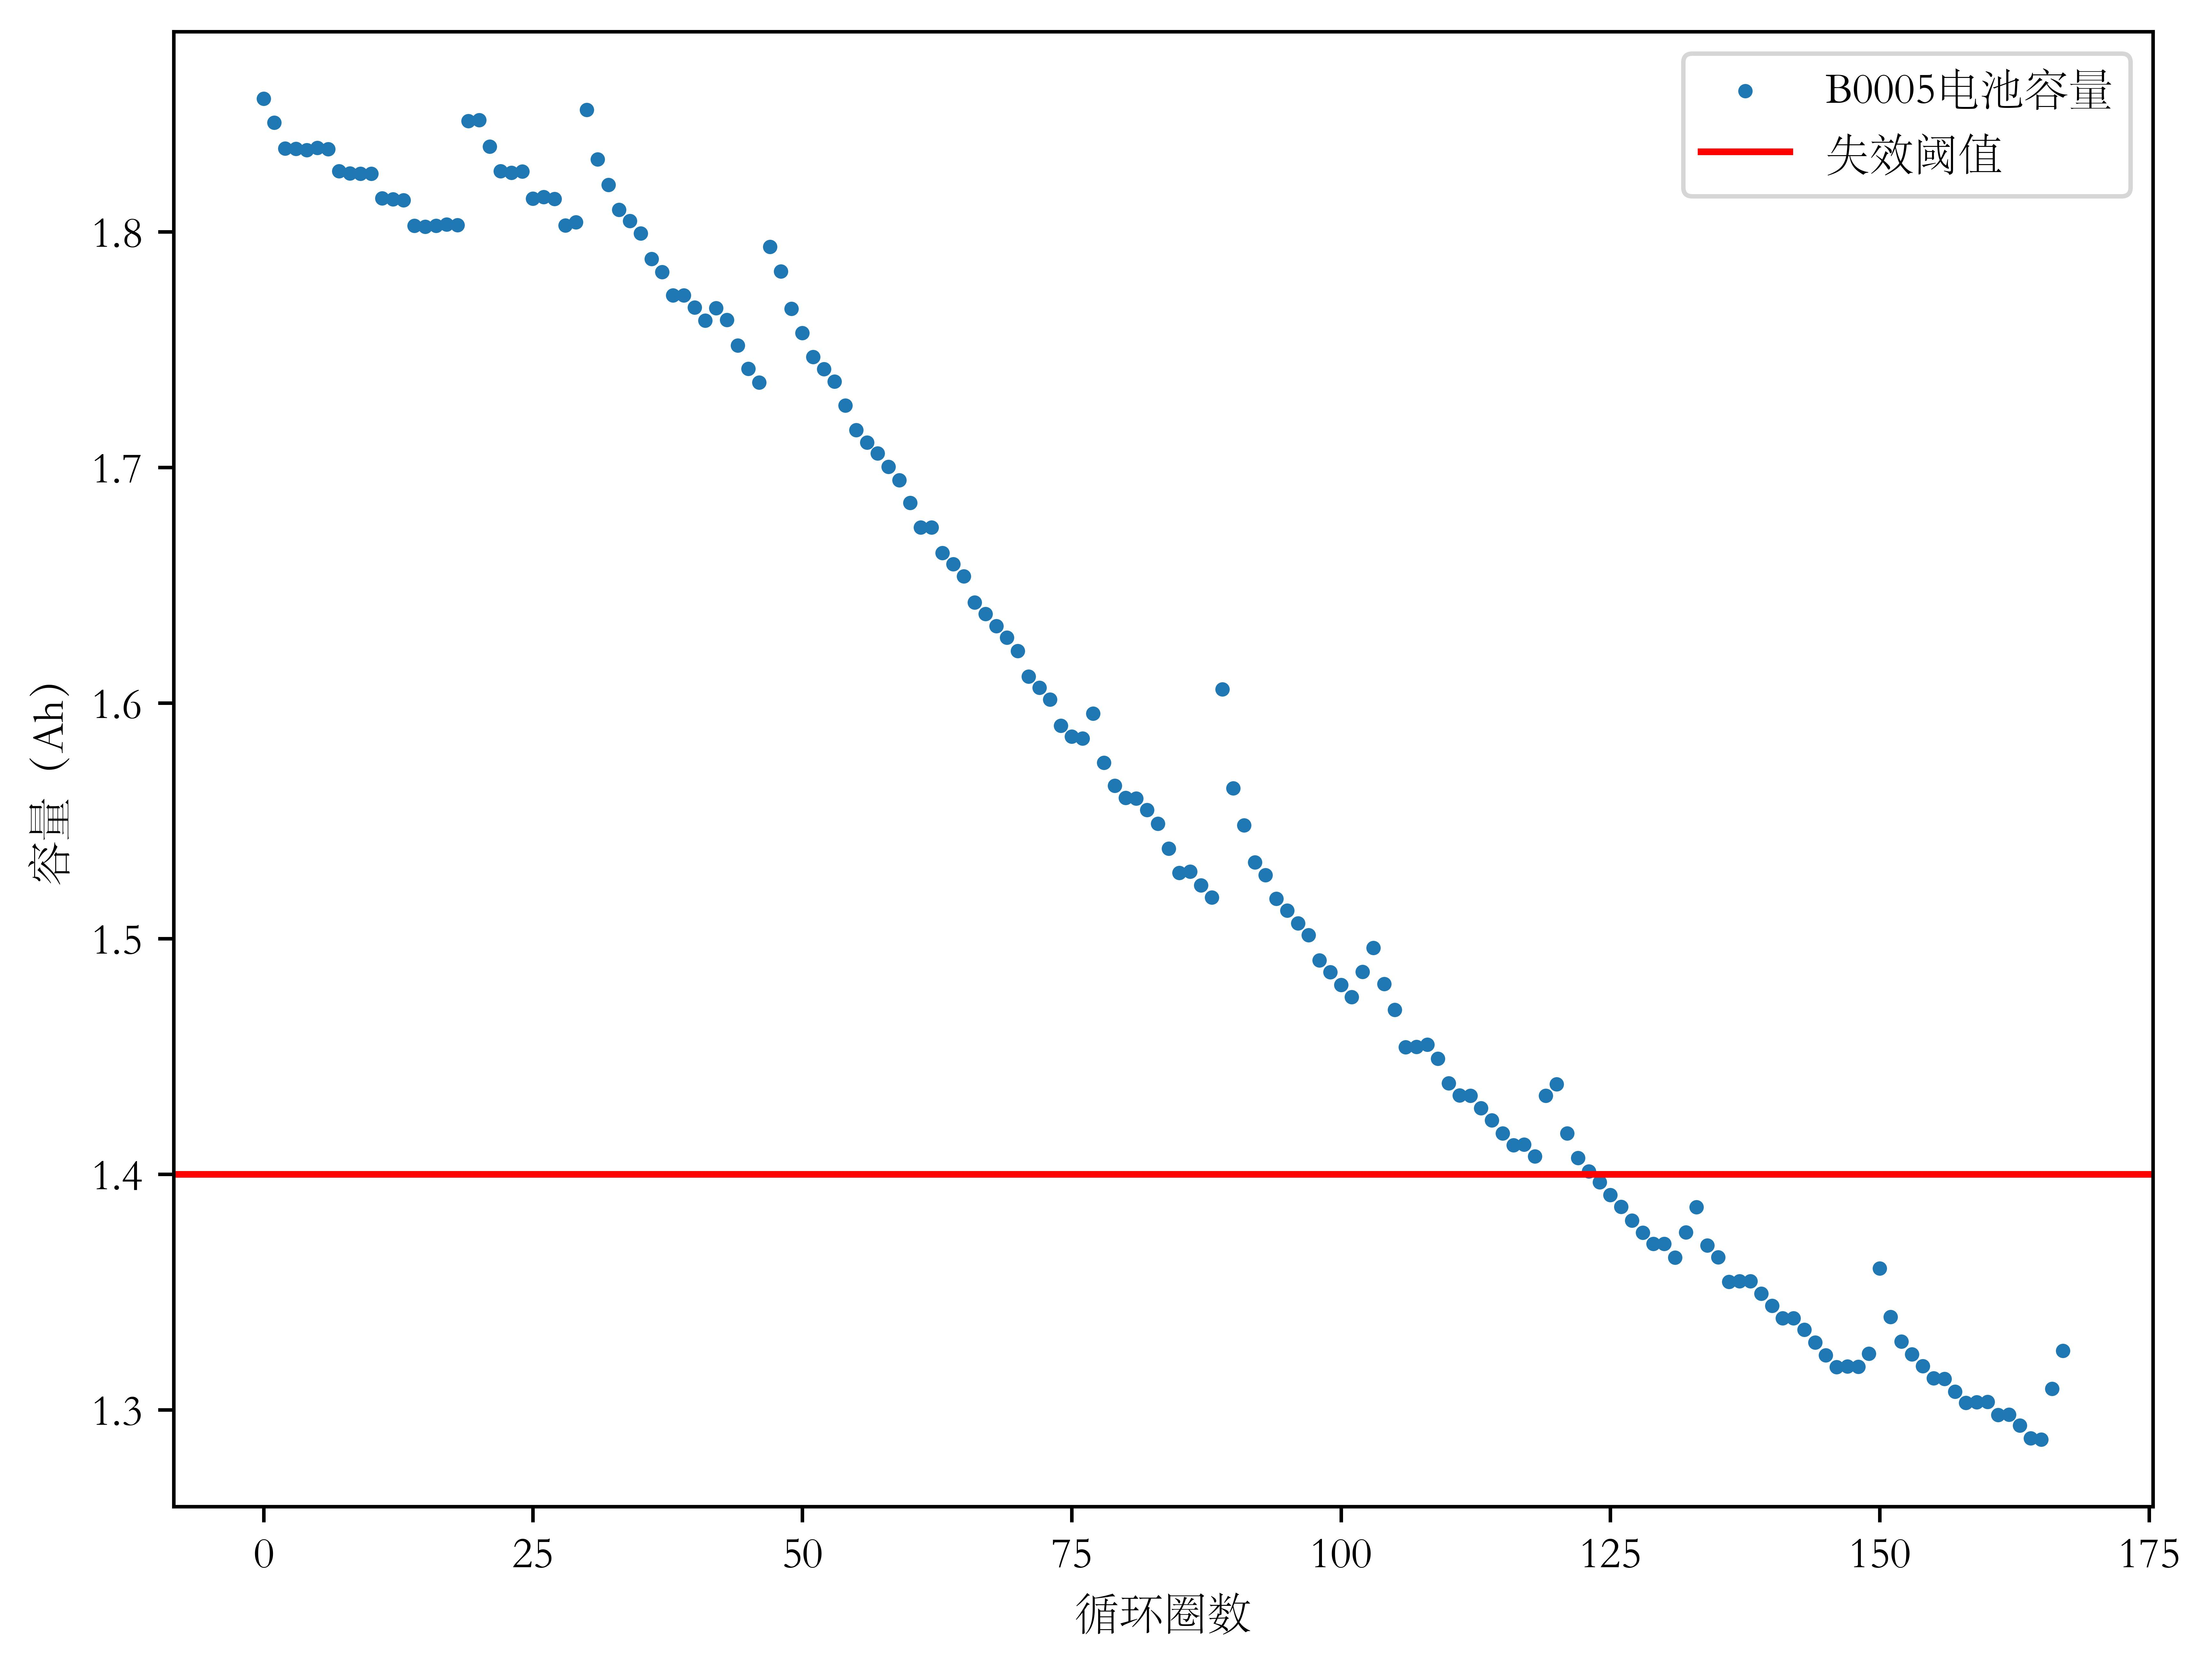
\includegraphics[width=0.25\textwidth]{figures/nasa_B0005_failure_threshold.jpg}}
		\subfloat[RUL]
		{\label{fig:subfig2}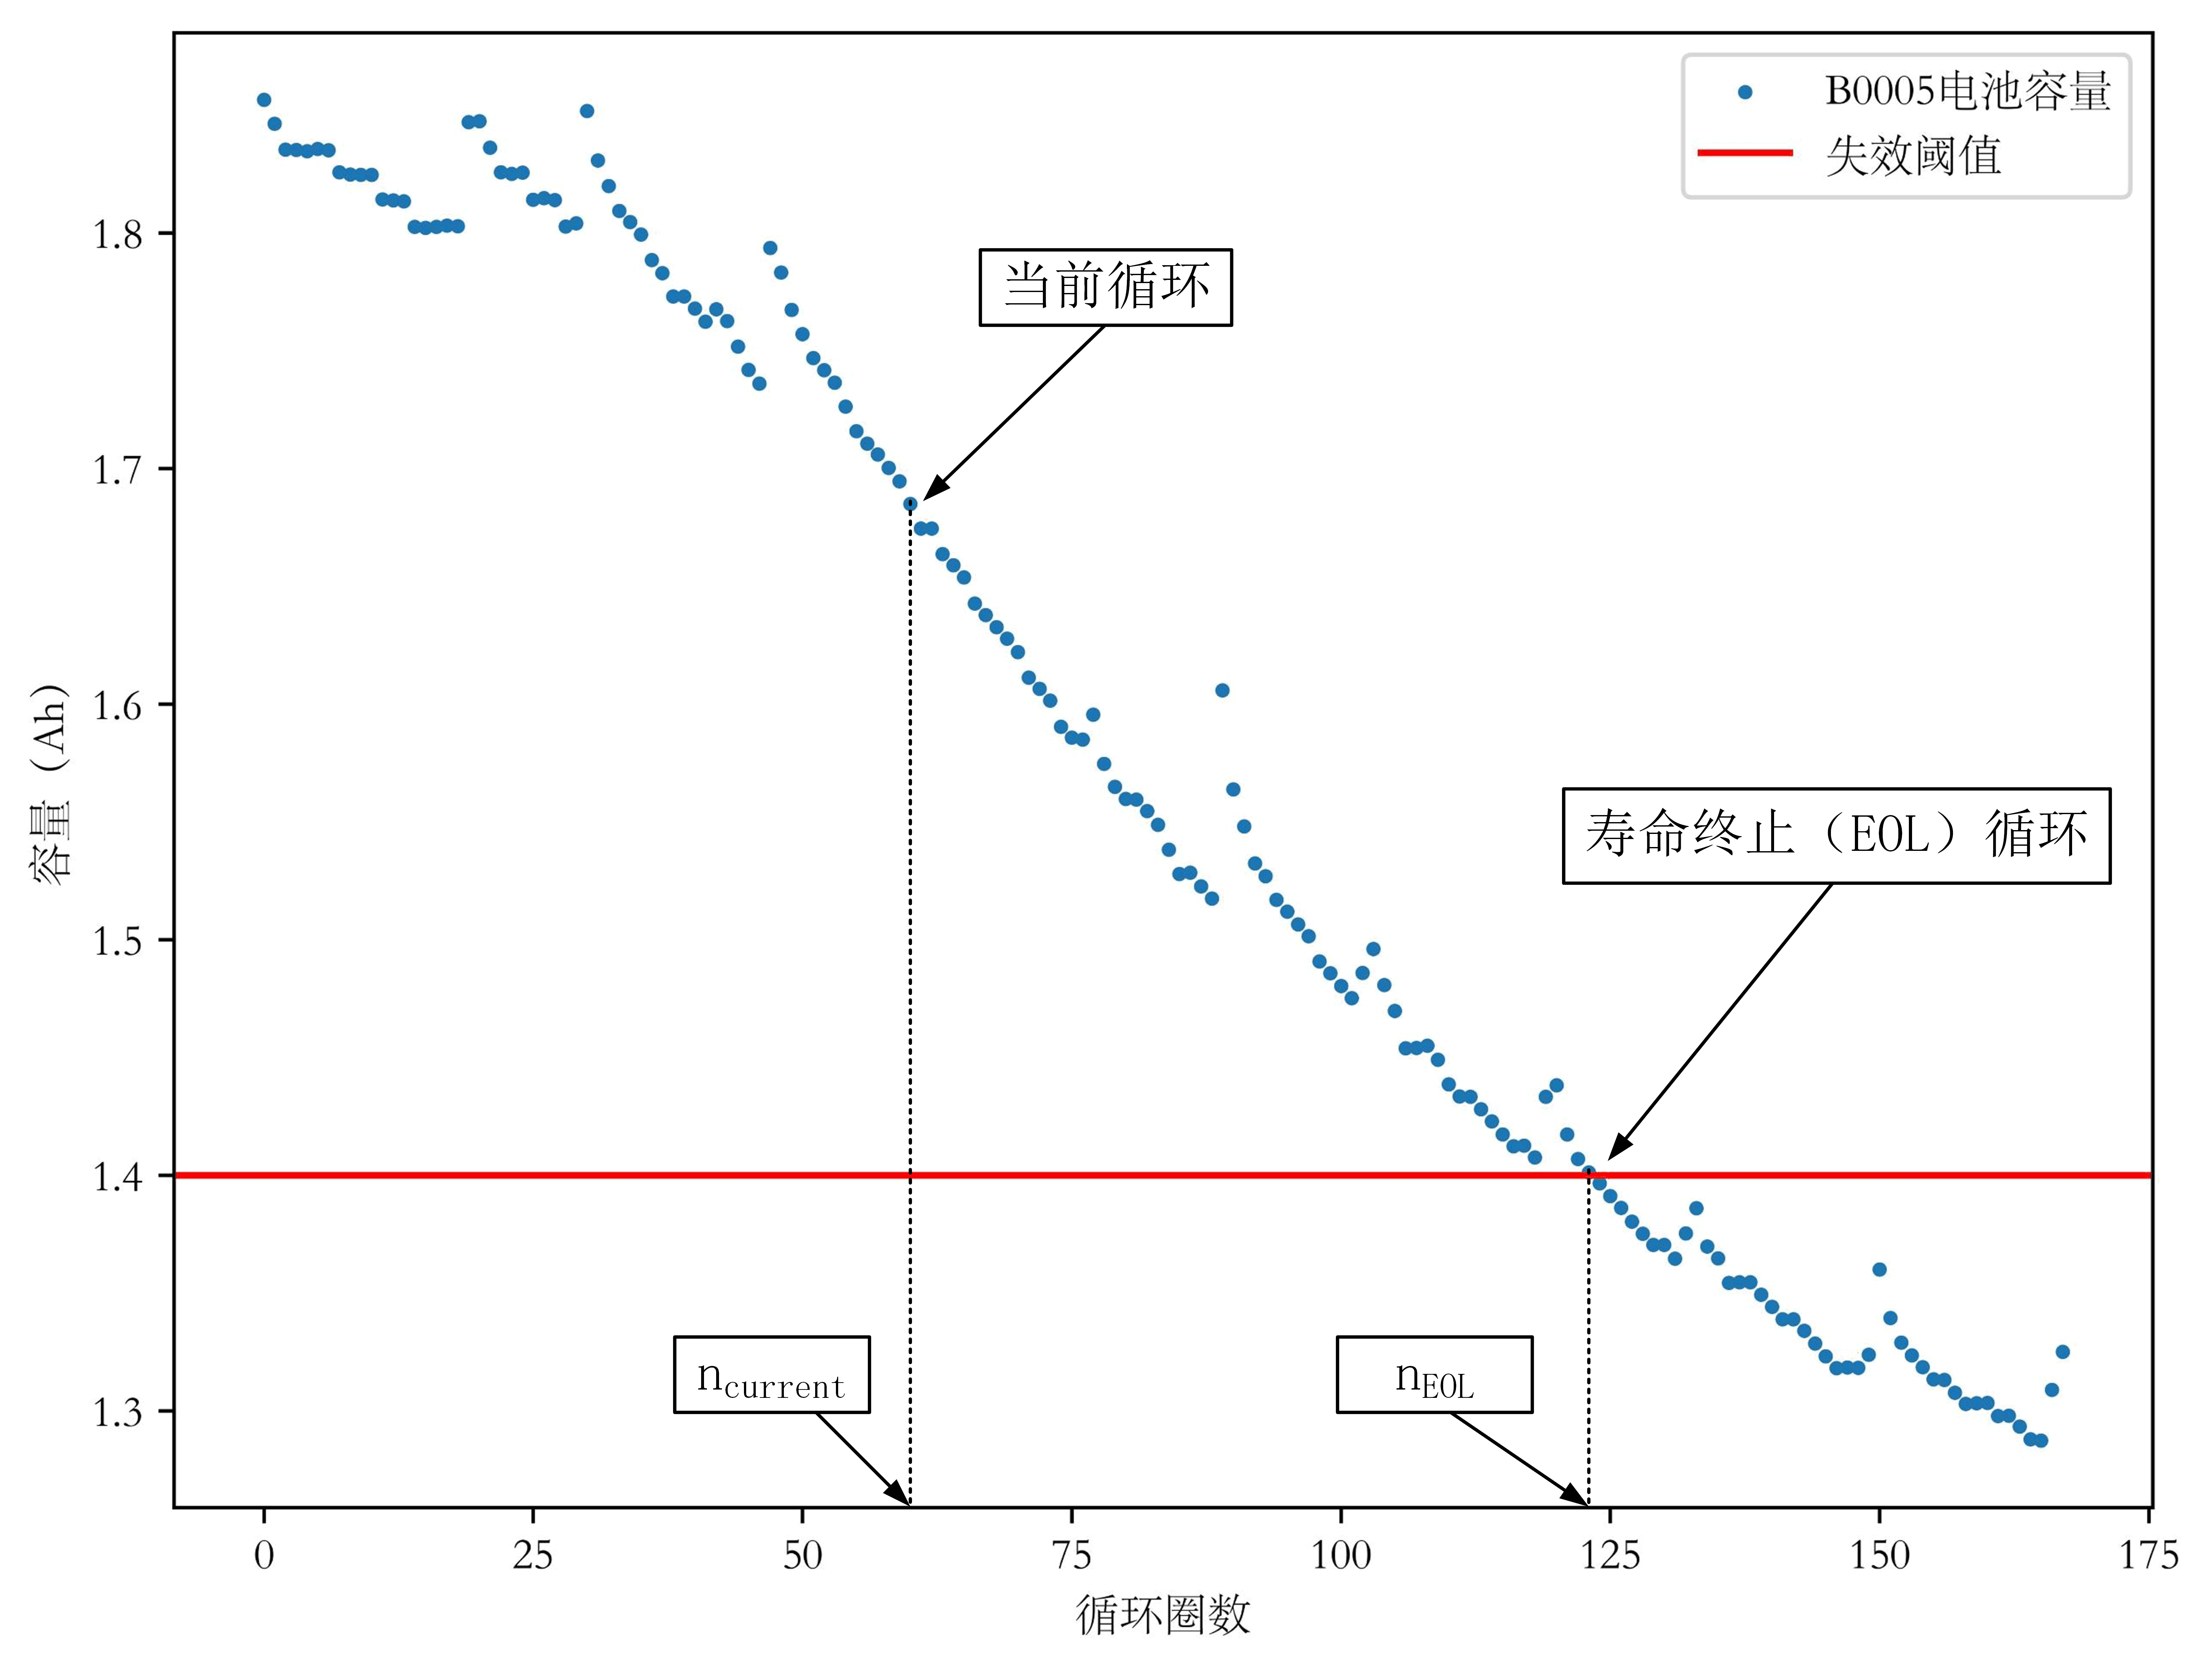
\includegraphics[width=0.25\textwidth]{figures/RUL.png}}
		\subfloat[SOC]
		{\label{fig:subfig3}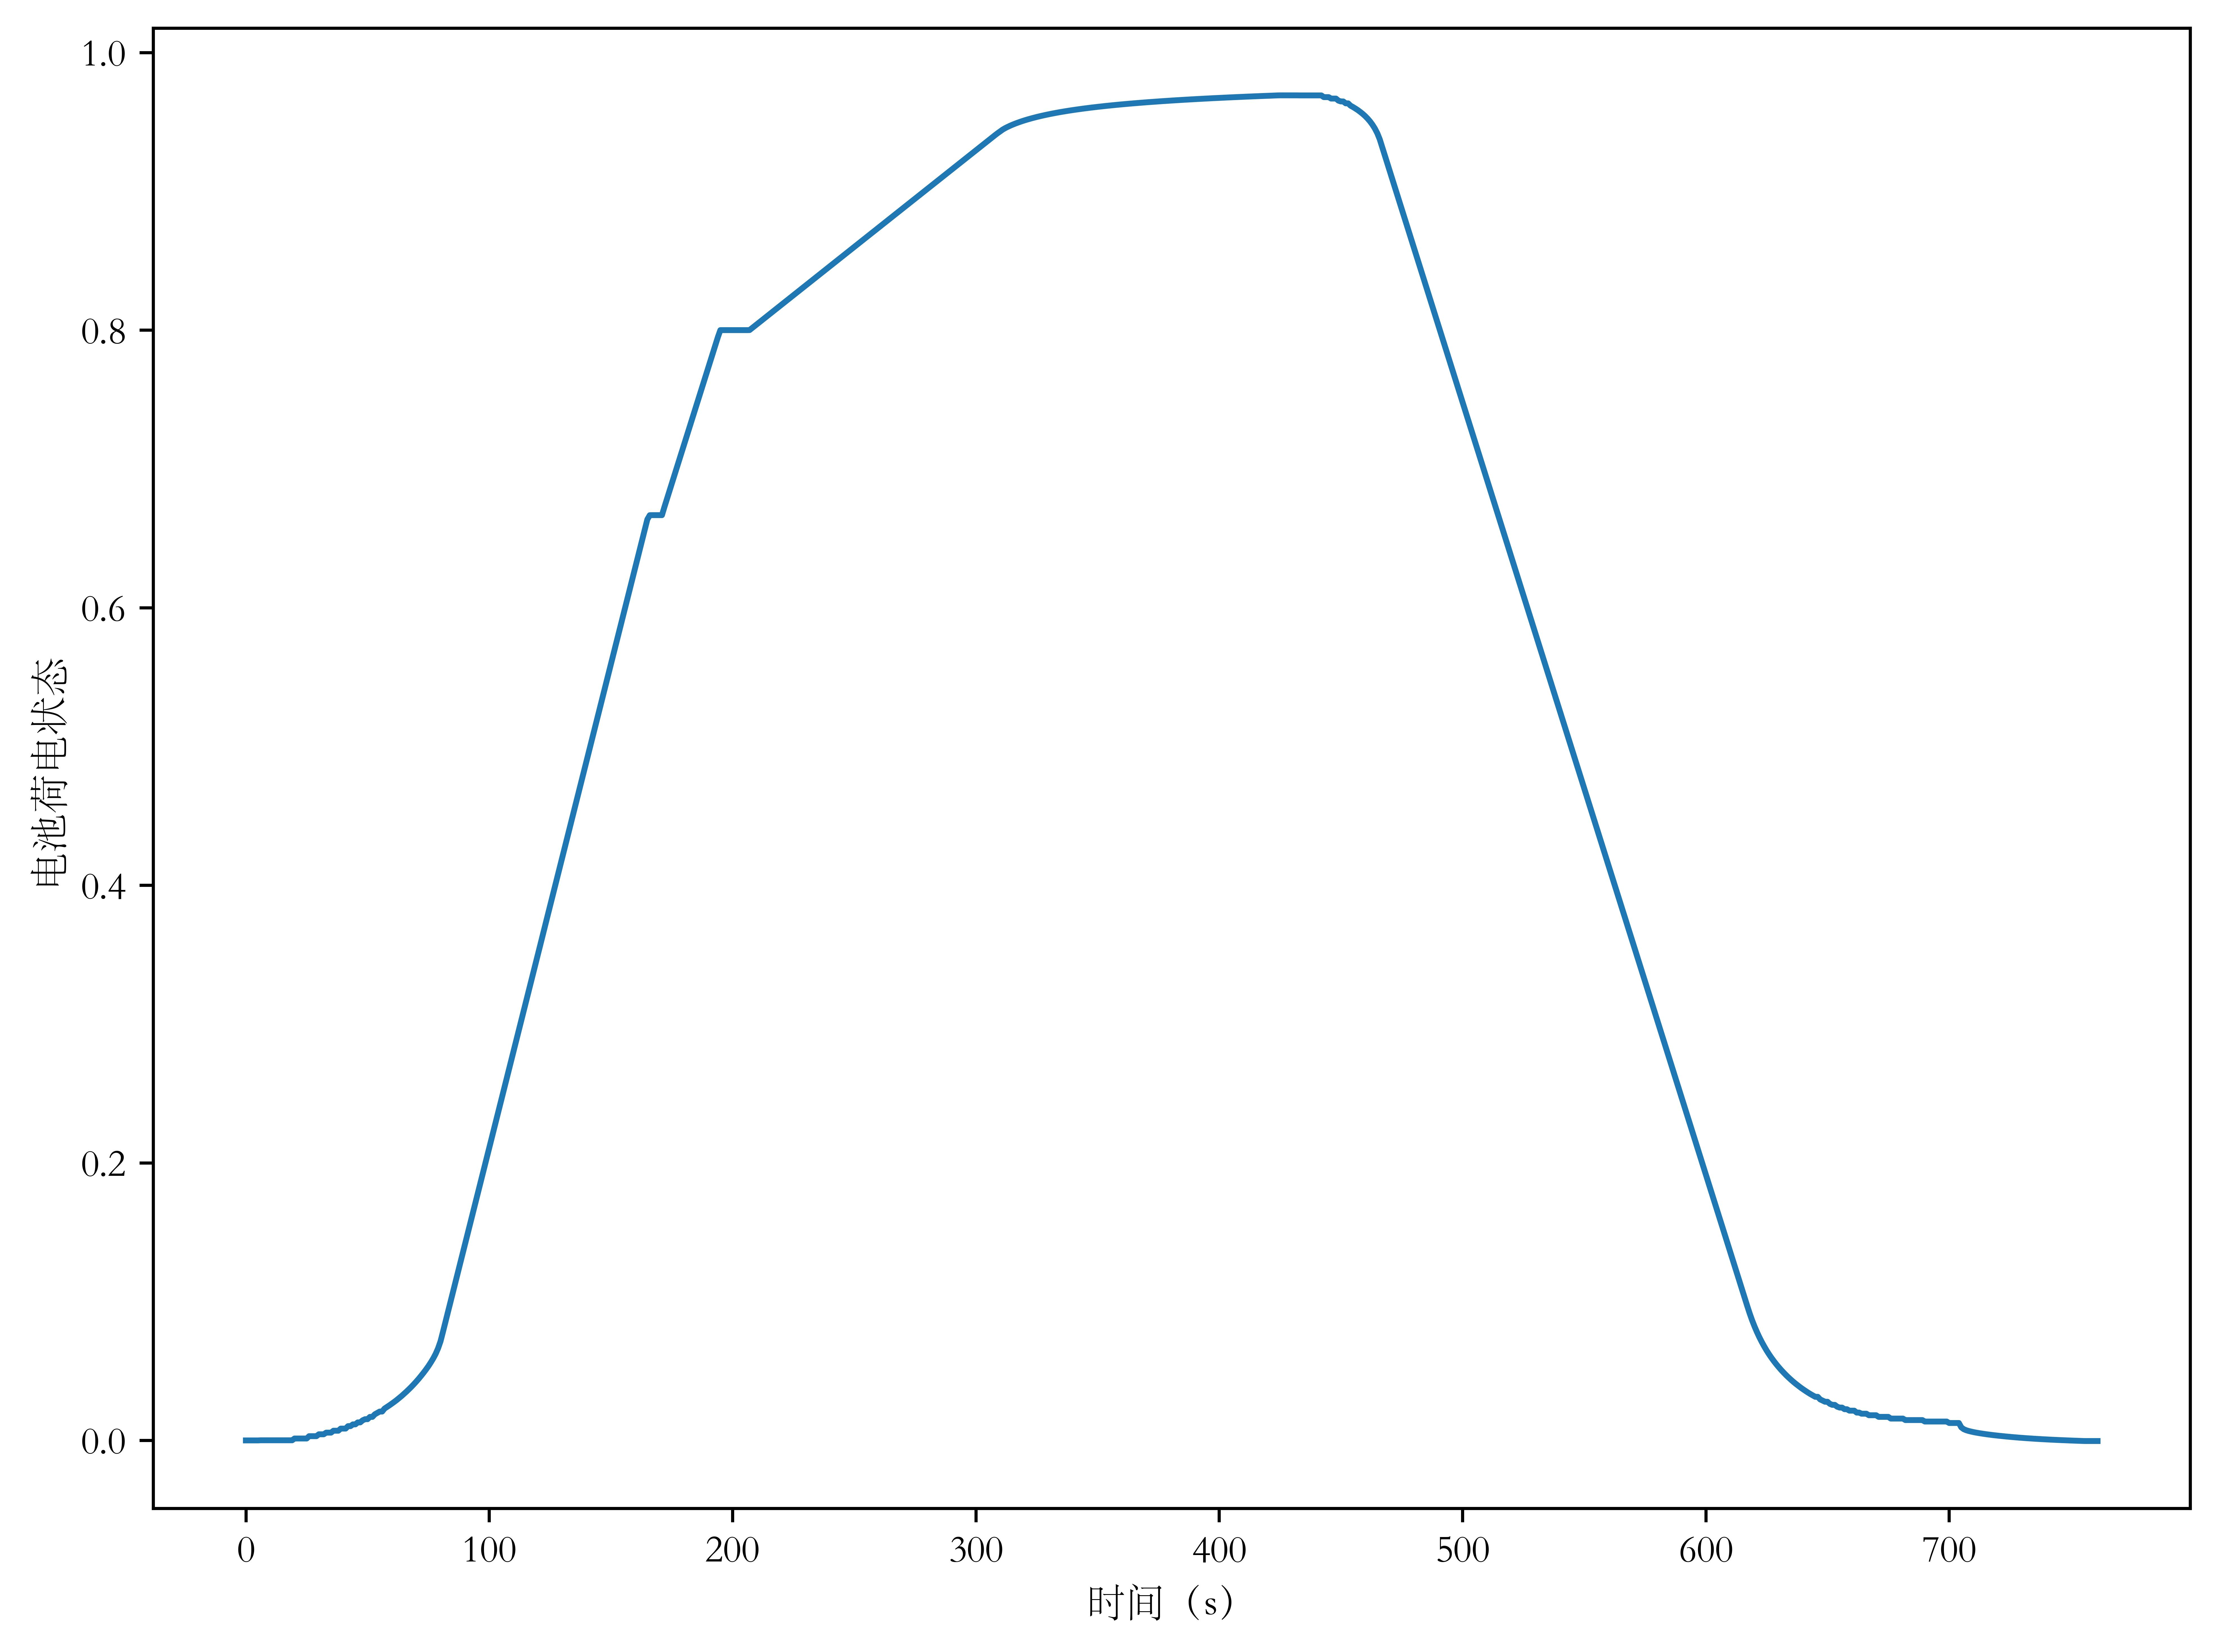
\includegraphics[width=0.25\textwidth]{figures/tri_b3c0_soc.jpg}}
		\captionsetup{font=tiny}
		\caption{电池SOH、RUL和SOC示意图}
	\end{figure}
	\begin{description}
		\item[SOH]
			电池健康状态,使用电池放电容量表征,描述电池性能退化状态,$SOH = \frac{Q_{max}}{Q_{nominal}} \times 100\%$
		\item[RUL]
			电池剩余寿命,描述电池从当前循环到寿命终止(EOL)循环的过程,$RUL = n_{EOL} - n_{current}$
		\item[SOC]
			电池荷电状态,和SOH有相同的形式,描述电池电荷量,$SOC = \frac{Q_{remain}}{Q_{max}} \times 100\%$
	\end{description}
    \pdfnote{锂离子电池被广泛用在各种领域中,尤其是交通运输行业。锂离子电池作为动力电池的应用规模日益增大,一方面使得其工作过程中的安全性问题越发重要,另一方面由其退役分选和梯次利用产生的经济效益逐渐引起市场关注。\\(注意说明公式定义)\\为了实现电池应用的安全性目标,同时最大化其经济效益,需要实现电池管理系统(BMS),电池健康状态(SOH)和电池剩余寿命(RUL)是其中两个重要的电池状态参数。SOH表征电池性能退化情况,RUL描述电池从某个循环到寿命终止(EOL)循环的过程。\\这里展示的电池荷电状态(SOC)是另一个重要状态参量,SOC不是本文研究对象,但其定义反映了SOH的重要意义。\\SOH和RUL都是难以直接测量的状态参数,需要通过间接手段估计和预测。主流的预测模型基于电池工作机理,这种方式需要大量先验知识、需要求解复杂的微分方程同时泛化能力交叉。本文使用数据驱动方法,以电池充放电数据为输入建立估计/预测模型。\\本文围绕电池SOH和RUL展开,分为三个部分。}
\end{frame}

\section{建模和实验}

\subsection{基于电池容量历史退化数据的SOH估计}

\begin{frame}
	\begin{figure}[htbp]
		\centering
		\subfloat[CALCE\_CS2\_35电池上的SOH估计结果]
		{\label{fig:subfig1}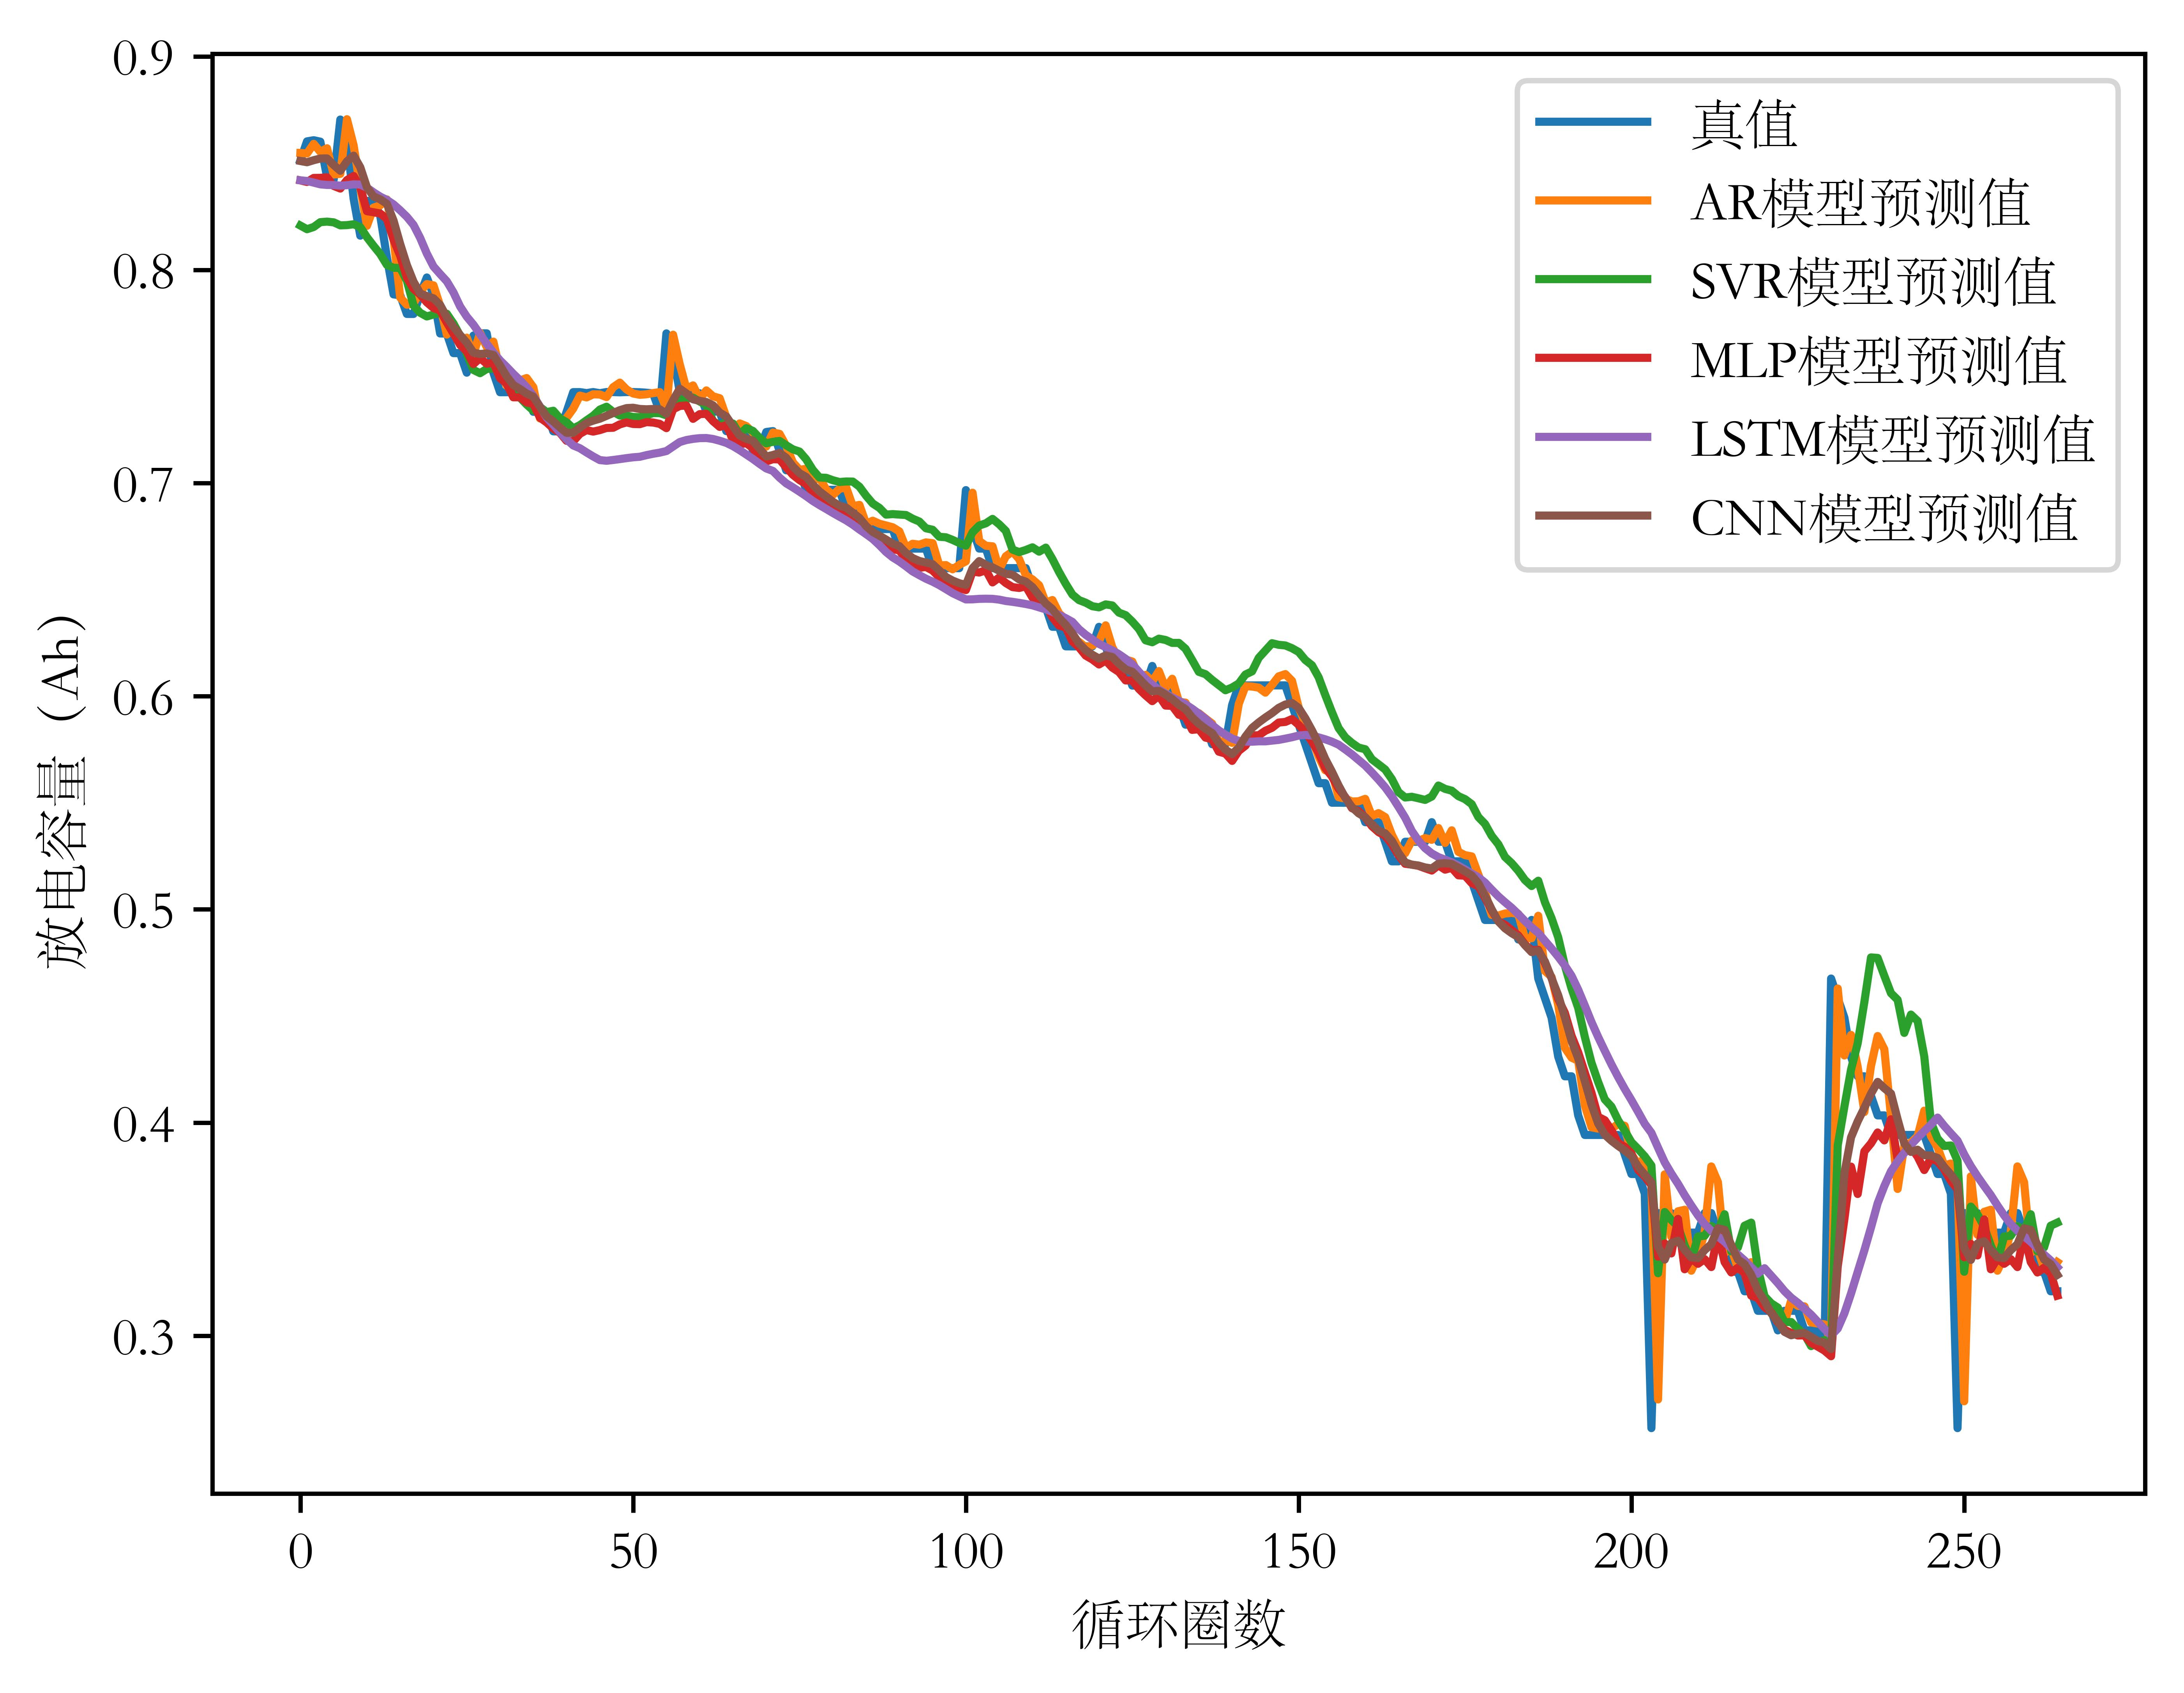
\includegraphics[width=0.45\textwidth]{figures/soh_cap/slide_figure_calce.jpg}}
		\subfloat[NASA\_PCoE\_B0005电池上的SOH估计结果]
		{\label{fig:subfig2}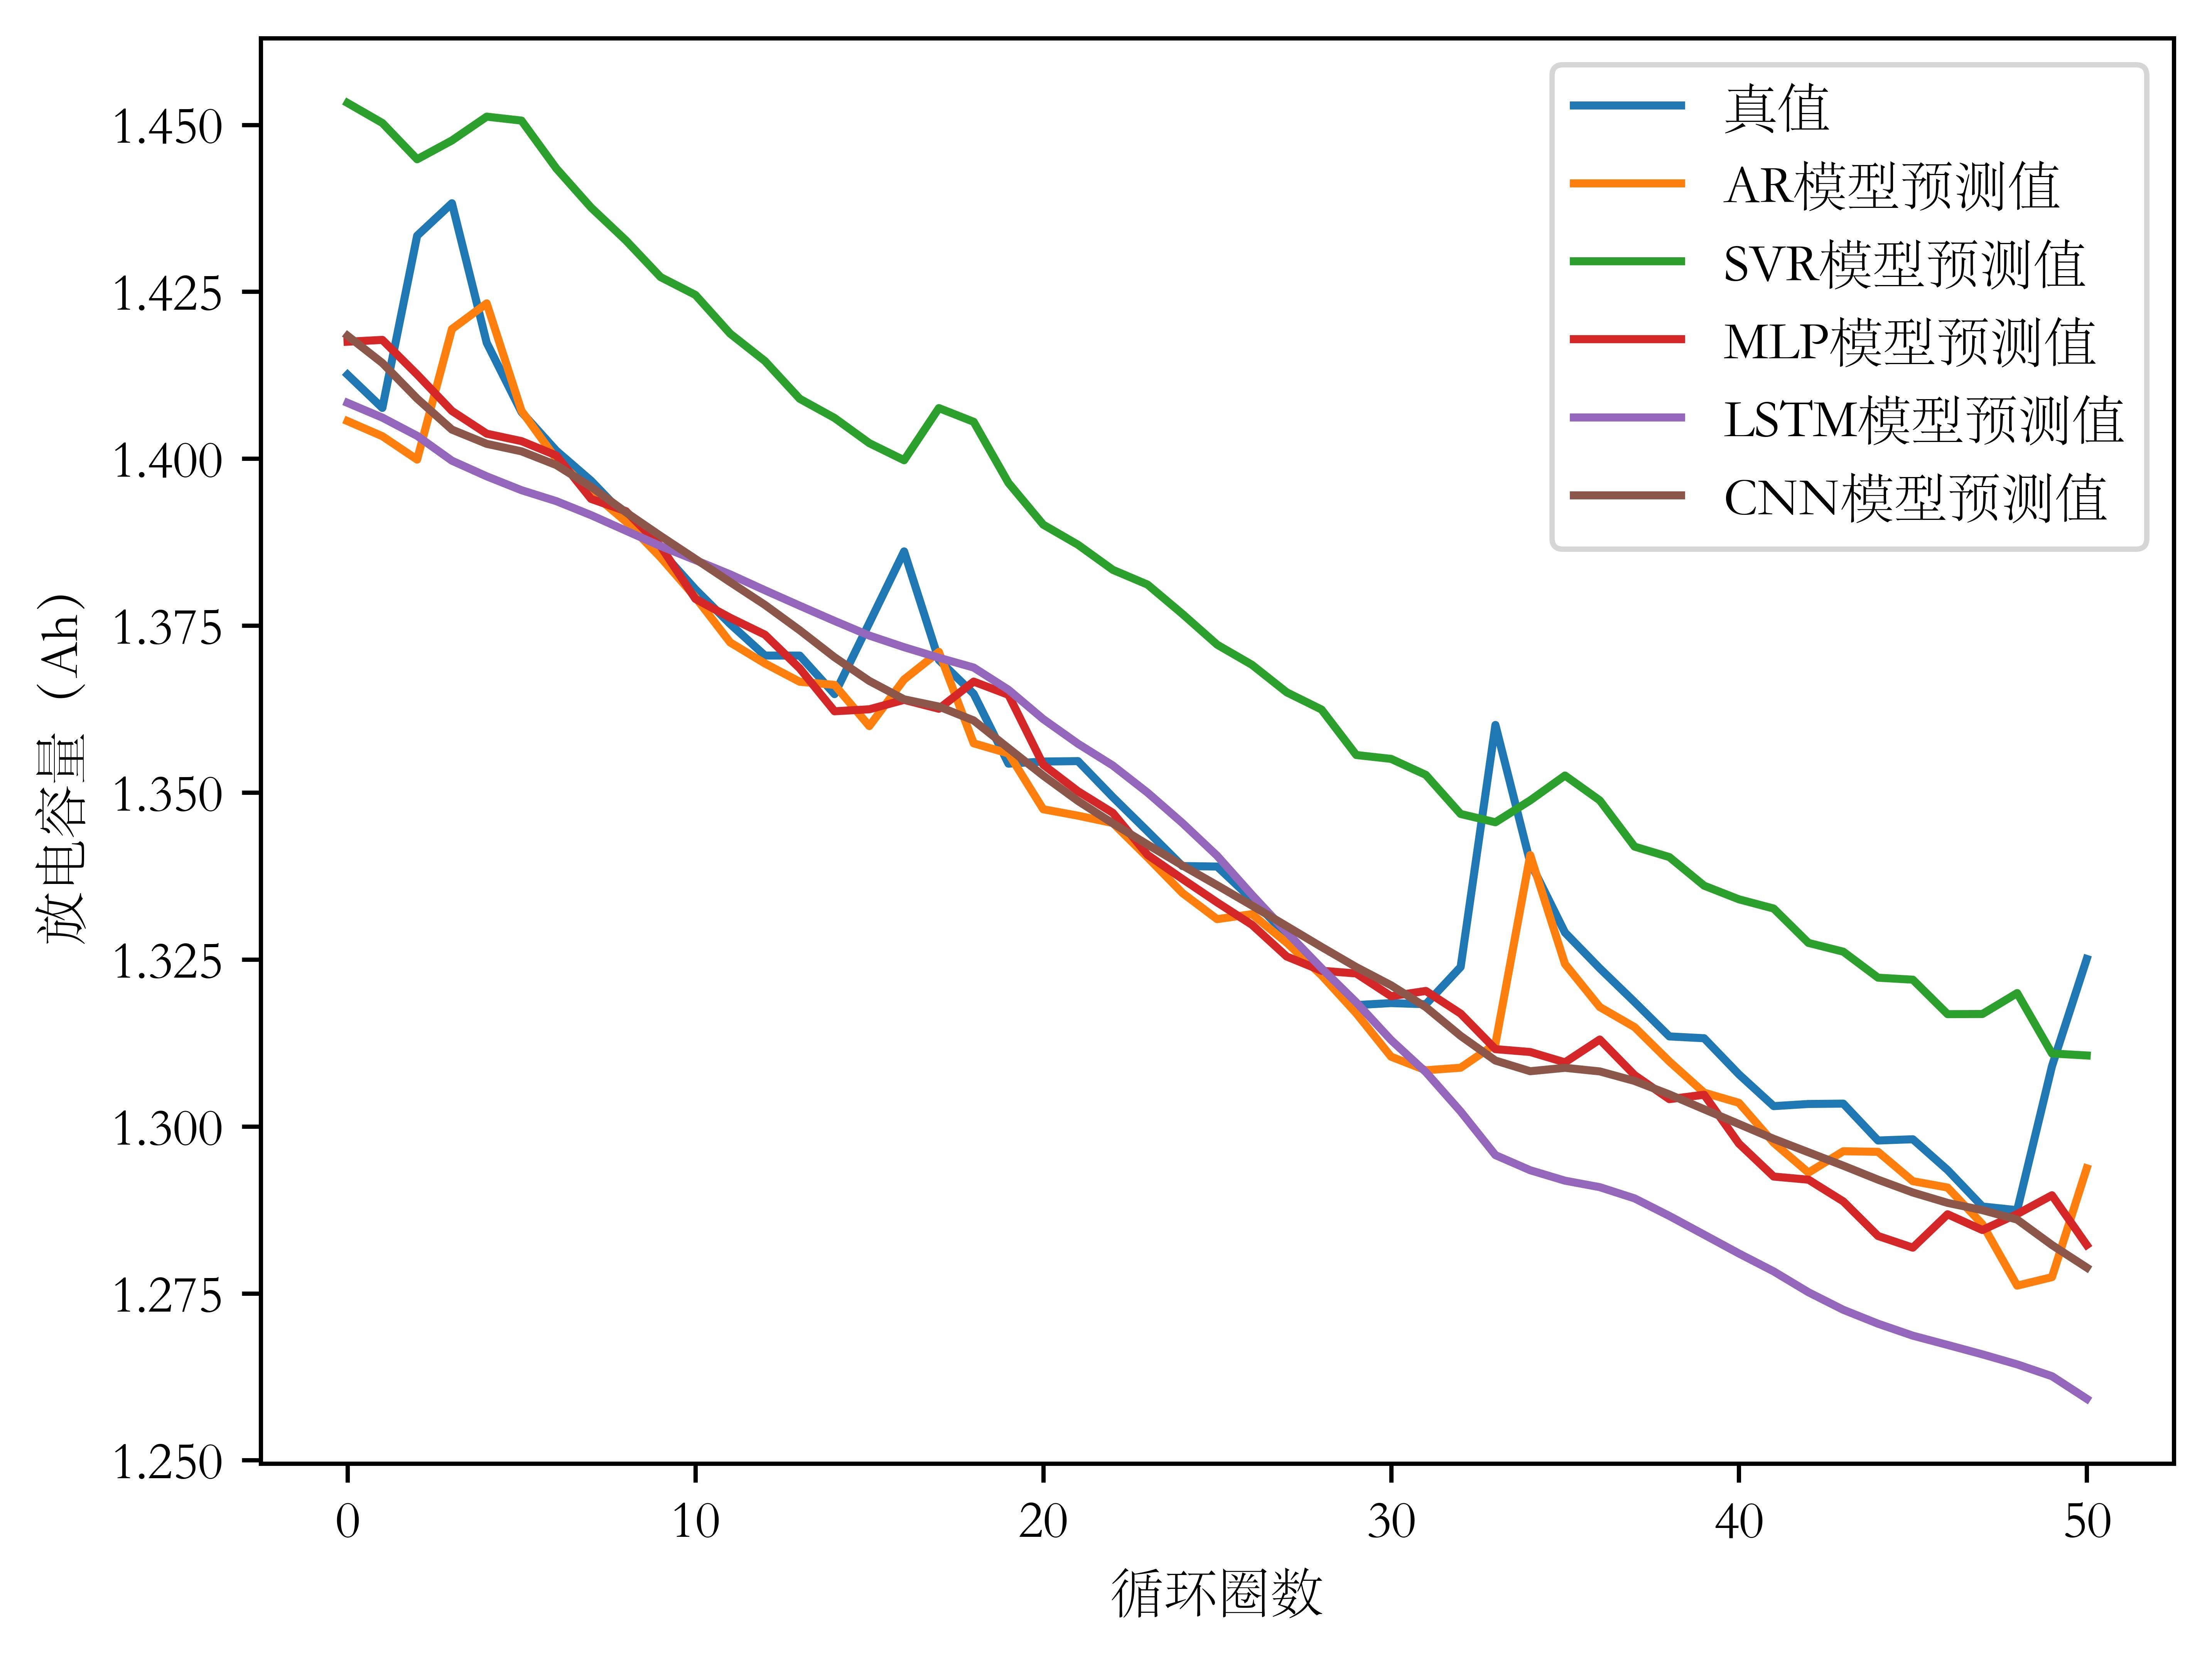
\includegraphics[width=0.45\textwidth]{figures/soh_cap/slide_figure_nasa.jpg}}
		\captionsetup{font=tiny}
		\caption{五种模型的SOH估计结果示意图}
	\end{figure}
	\begin{itemize}
		\item 在CALCE数据集(包含4颗电池的循环数据)和NASA PCoE数据集(包含4颗电池的循环数据)上开展实验,采用留一法划分数据集
		\item 受篇幅限制,展示在CALCE\_CS2\_35电池和NASA\_PCoE\_B0005电池上的测试结果
	\end{itemize}
	\pdfnote{本课题的第一部分是基于历史容量退化数据的电池SOH估计。这一部分研究的目的在于验证数据驱动方法的可行性并比较不同模型的预测性能。\\这部分研究实现了5种模型,分别是自回归(AR)模型,支持向量回归(SVR)模型,多层感知机(MP)模型,长短期记忆神经网络(LSTM)模型和卷积神经网络(CNN)模型。\\以前16个循环的放电容量为输入估计当前循环的放电容量,5种模型在2个数据集上的预测结果示意如图。}
\end{frame}

\begin{frame}
	\begin{table}[]
		\centering
		\resizebox{\columnwidth}{!}{%
			\begin{tabular}{ccccccccccc}
				\toprule
				\multirow{2}{*}{评价指标} & \multicolumn{5}{c}{CALCE数据集} & \multicolumn{5}{c}{NASA PCoE数据集}                                                                                         \\
				                      & AR                           & SVR                              & MLP   & LSTM  & CNN               & AR                & SVR   & MLP   & LSTM  & CNN   \\
				\midrule
				平均MaxE                & \underline{0.116}            & 0.141                            & 0.147 & 0.152 & 0.142             & \underline{0.054} & 0.097 & 0.111 & 0.158 & 0.113 \\
				平均MAE                 & 0.010                        & 0.023                            & 0.009 & 0.028 & \underline{0.008} & \underline{0.008} & 0.033 & 0.019 & 0.041 & 0.020 \\
				平均RMSE                & 0.016                        & 0.028                            & 0.014 & 0.035 & \underline{0.013} & \underline{0.013} & 0.037 & 0.026 & 0.057 & 0.027 \\
				\bottomrule
			\end{tabular}%
		}
		\captionsetup{font=tiny}
		\caption{五种模型预测性能评估结果}
	\end{table}
	\begin{itemize}
		\item 五个模型均取得较高预测精度,使用数据驱动方法实现锂离子电池SOH估计具有可行性
		\item 对于短期时间序列预测问题,非隐状态模型(AR、SVR、MLP和CNN)的预测精度优于隐状态模型(LSTM)
	\end{itemize}
	\pdfnote{这一页展示了五种数据驱动方法在两个数据集上的预测性能,使用最大误差(MaxE)、平均绝对误差(MAE)和均方根误差(RMSE)作为评价指标。\\由表,五种模型均取得较高的预测精度,实验结果证明了数据驱动方法的可行性。\\同时,比较模型的具体性能,对于短期时间序列预测问题,非隐状态模型(AR、SVR、MLP和CNN)的预测精度优于隐状态模型(LSTM)。}
\end{frame}

\subsection{基于电池充放电直接测量量的SOH估计}

\begin{frame}
	\begin{figure}[htbp]
		\centering
		\subfloat[VIT输入,无变换]
		{\label{fig:subfig1}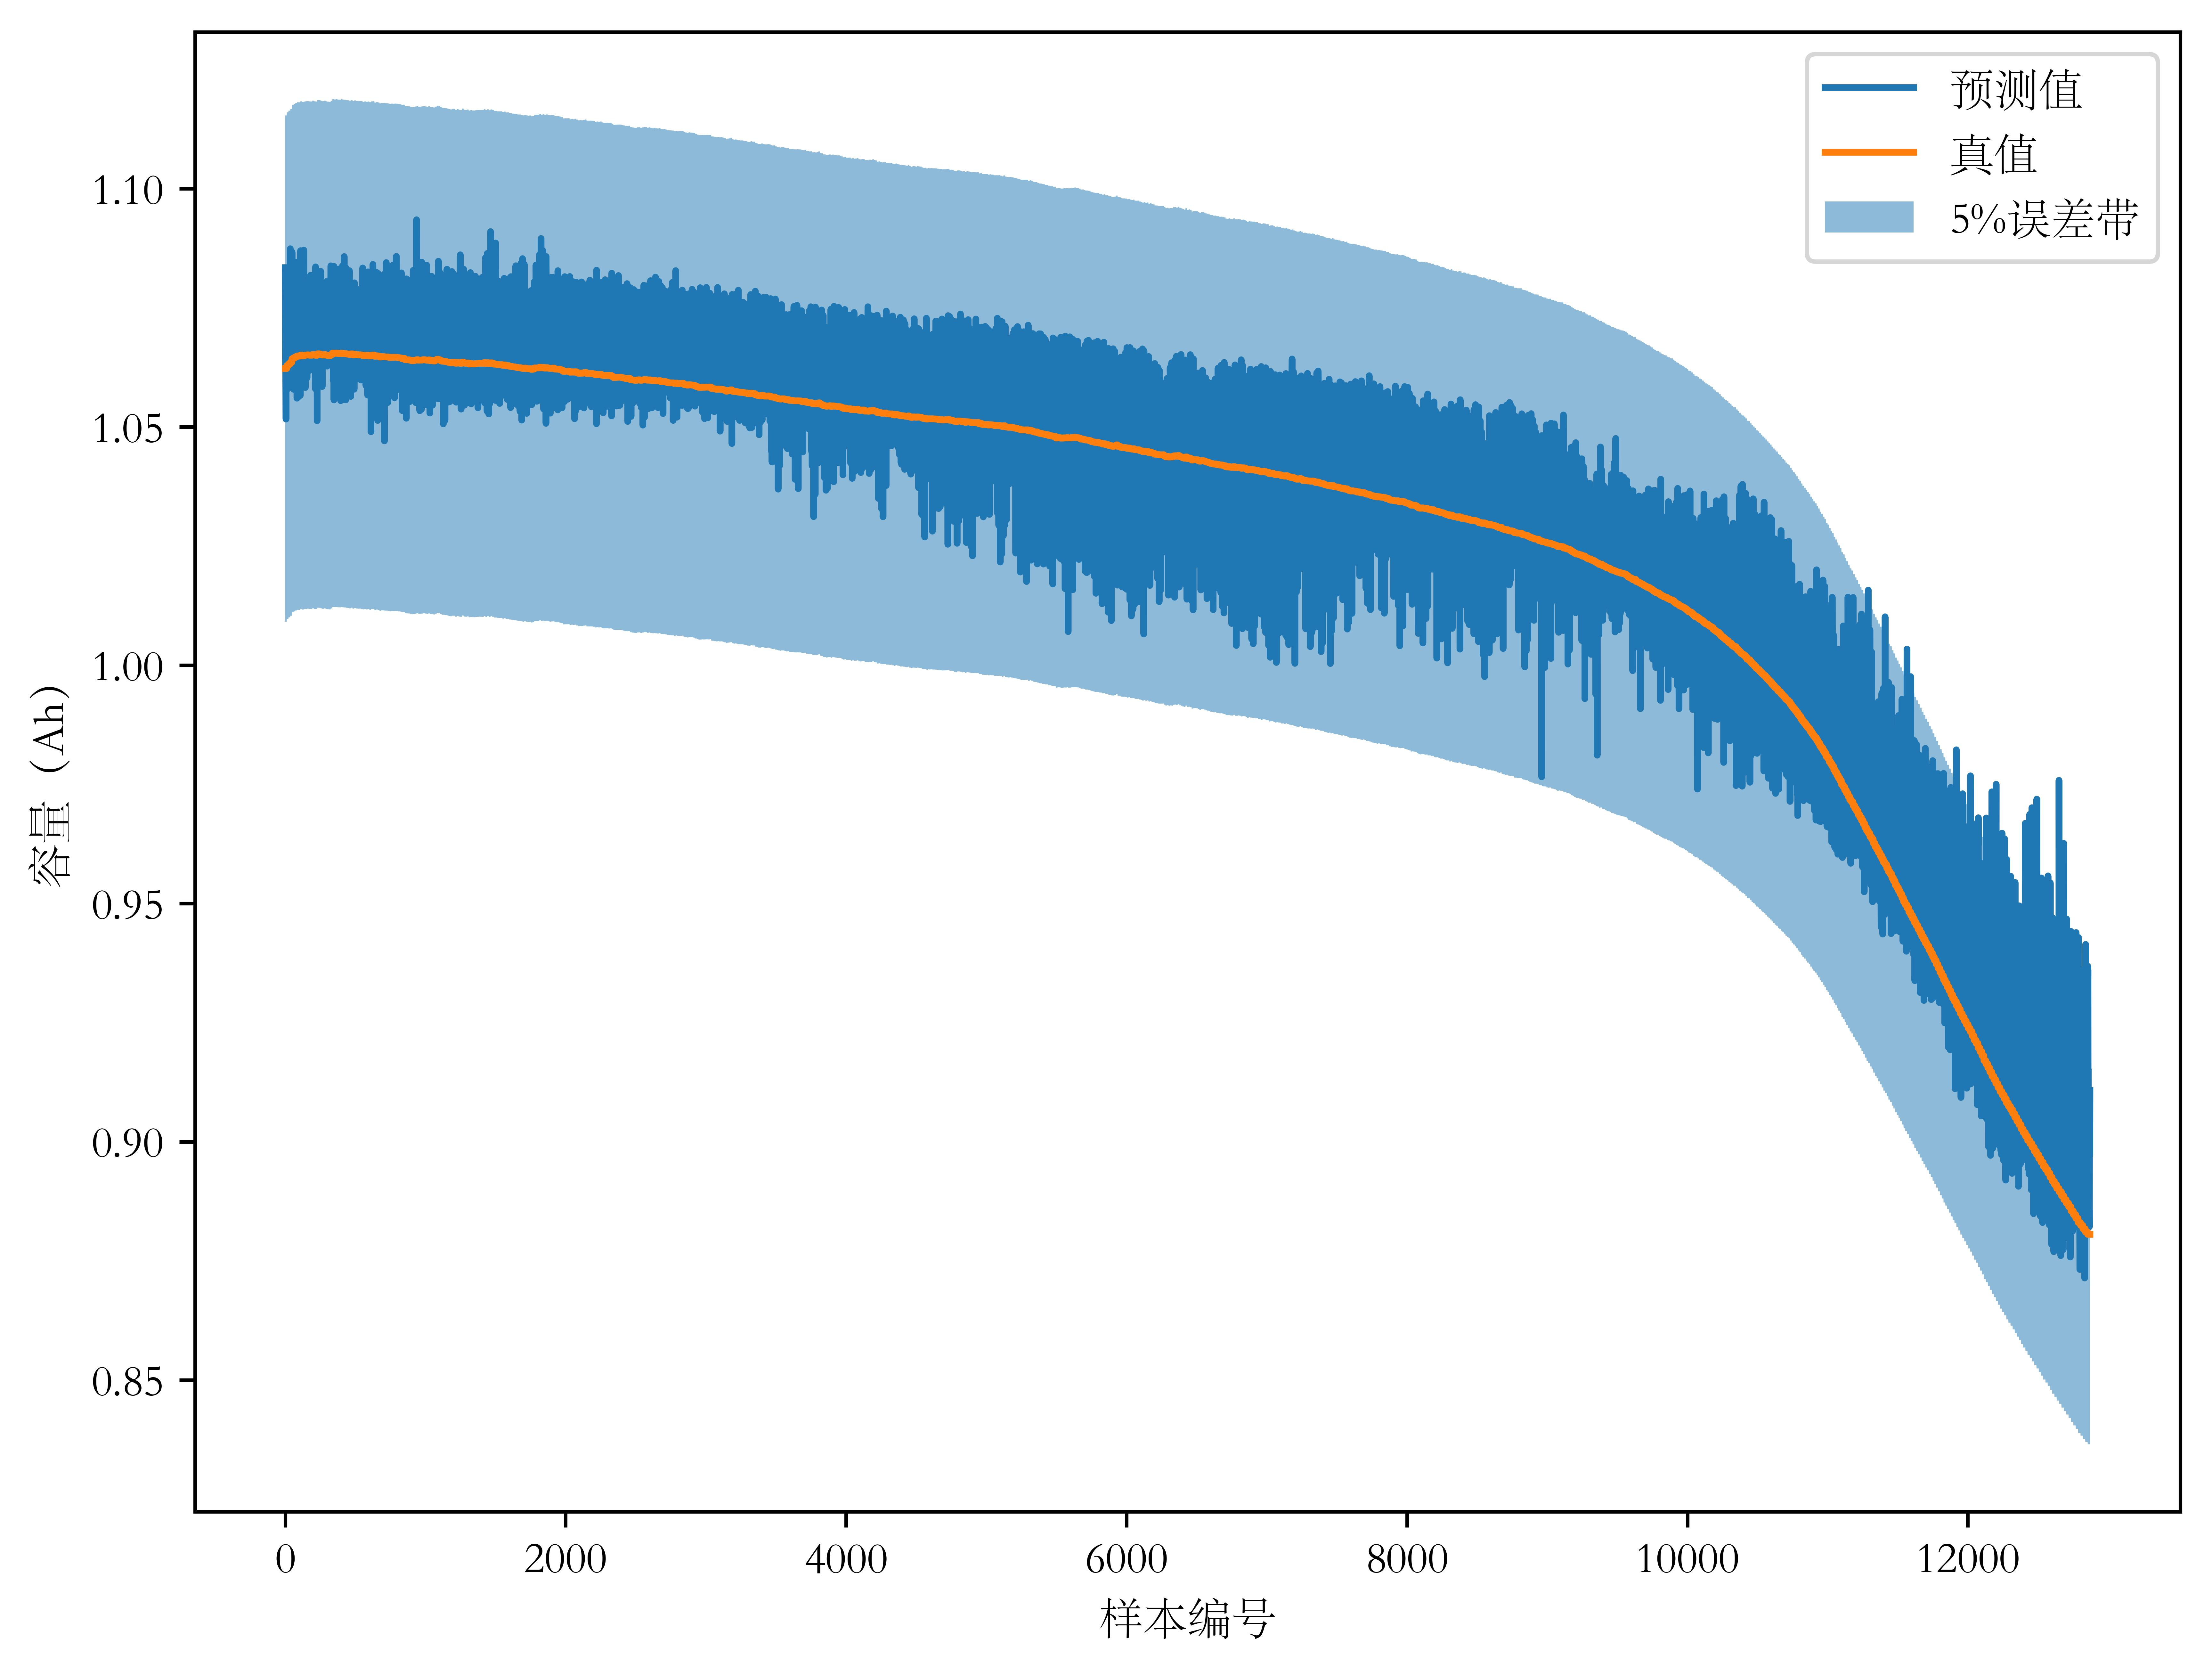
\includegraphics[width=0.25\textwidth]{figures/soh_vitq/tri_group1_cell4_cnn_vit.jpg}}
		\subfloat[VIq输入,无变换]
		{\label{fig:subfig2}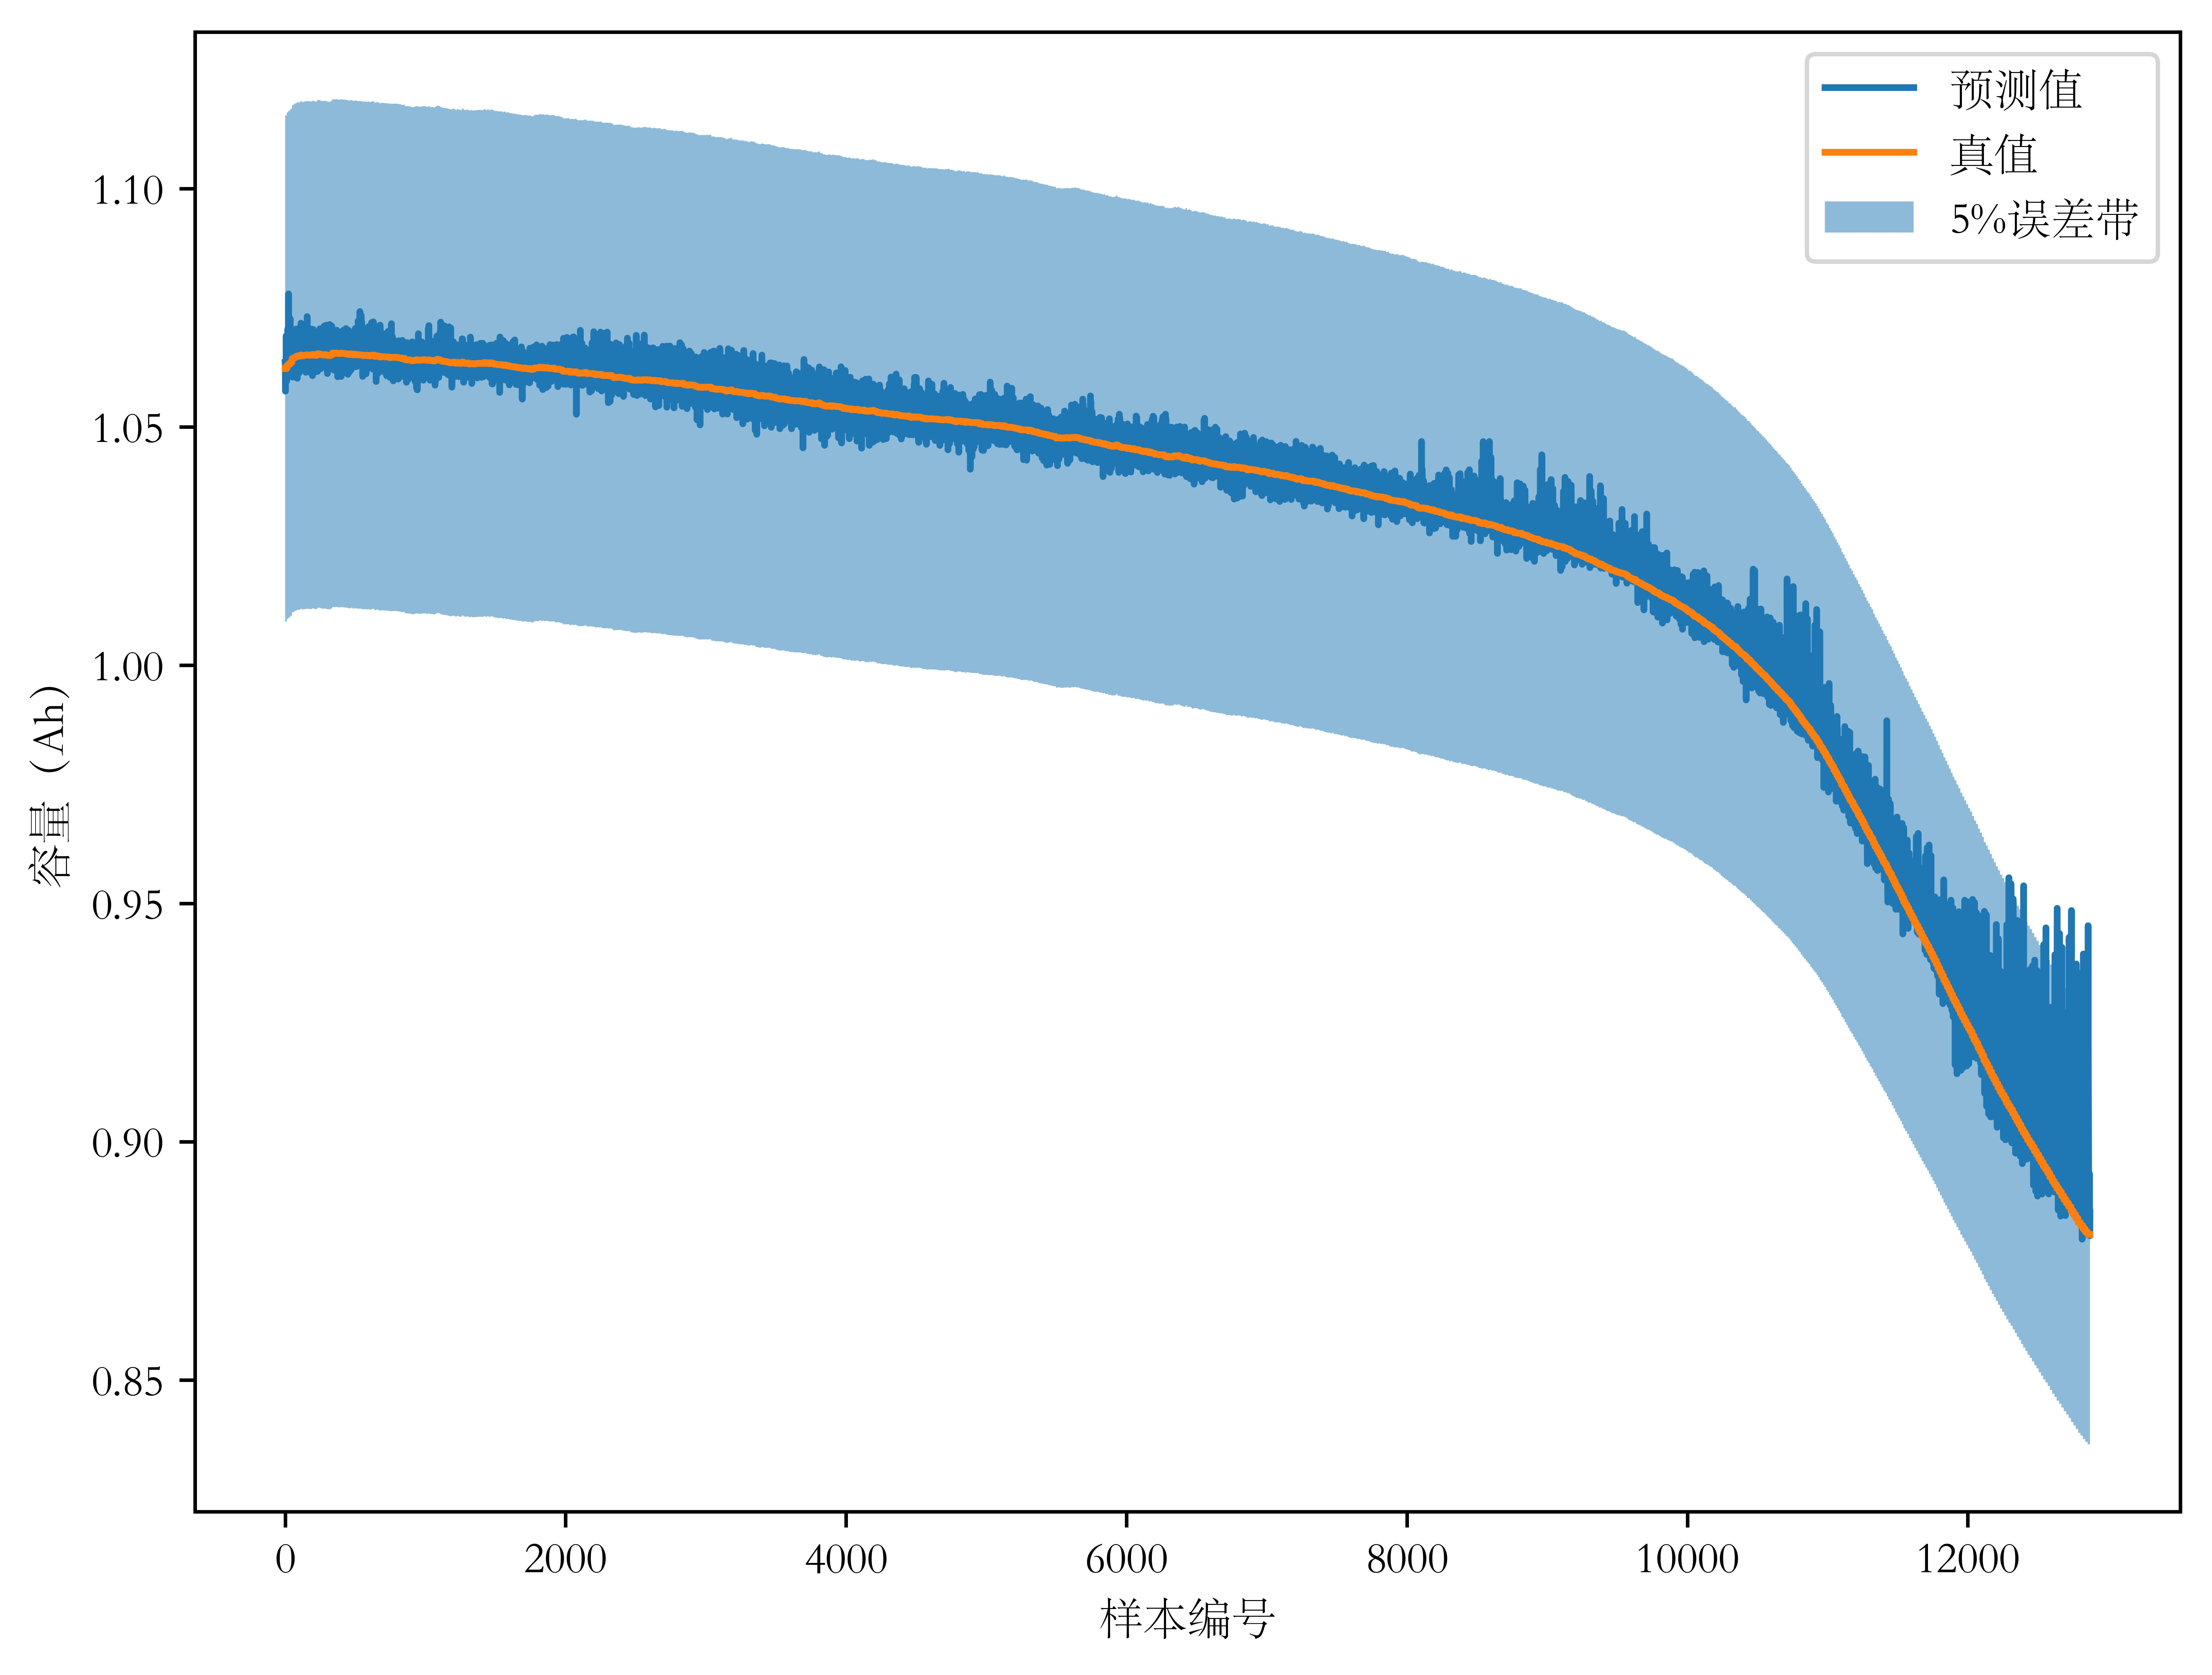
\includegraphics[width=0.25\textwidth]{figures/soh_vitq/tri_group1_cell4_cnn_viq.jpg}}
		\subfloat[VIT输入,有变换]
		{\label{fig:subfig3}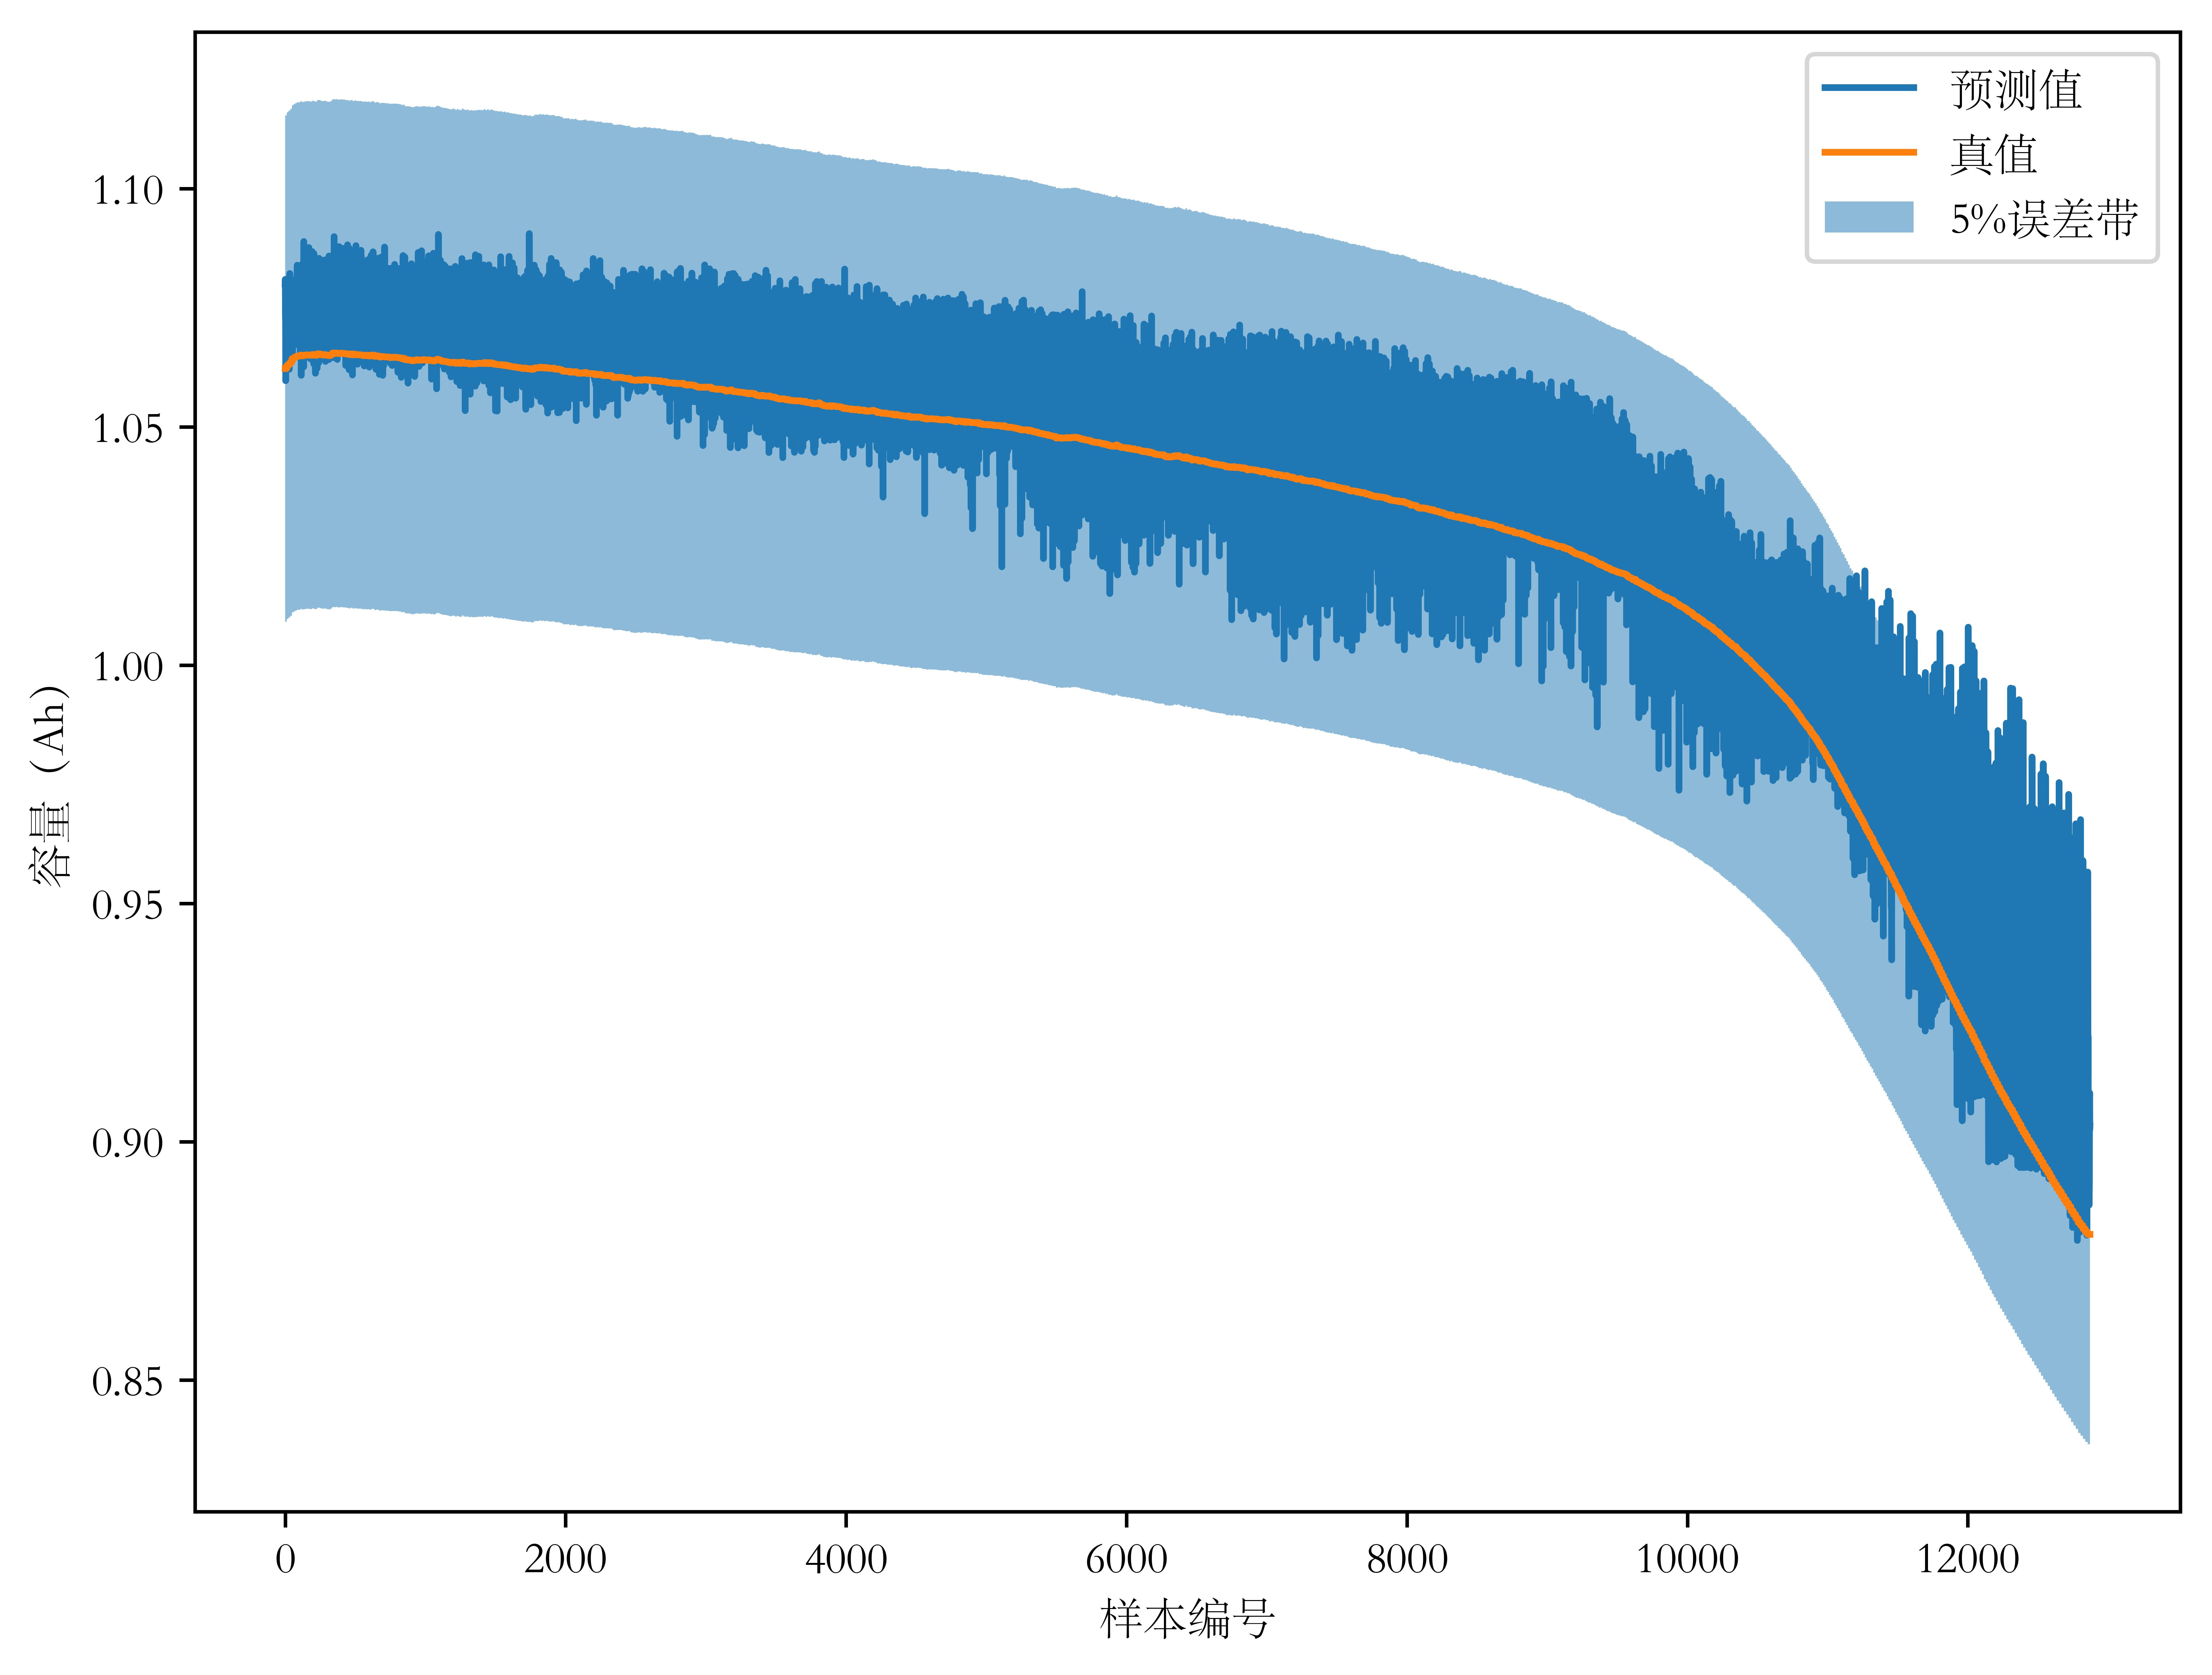
\includegraphics[width=0.25\textwidth]{figures/soh_vitq/tri_group1_cell4_cnn_vit_trans.jpg}}
		\subfloat[VIq输入,有变换]
		{\label{fig:subfig4}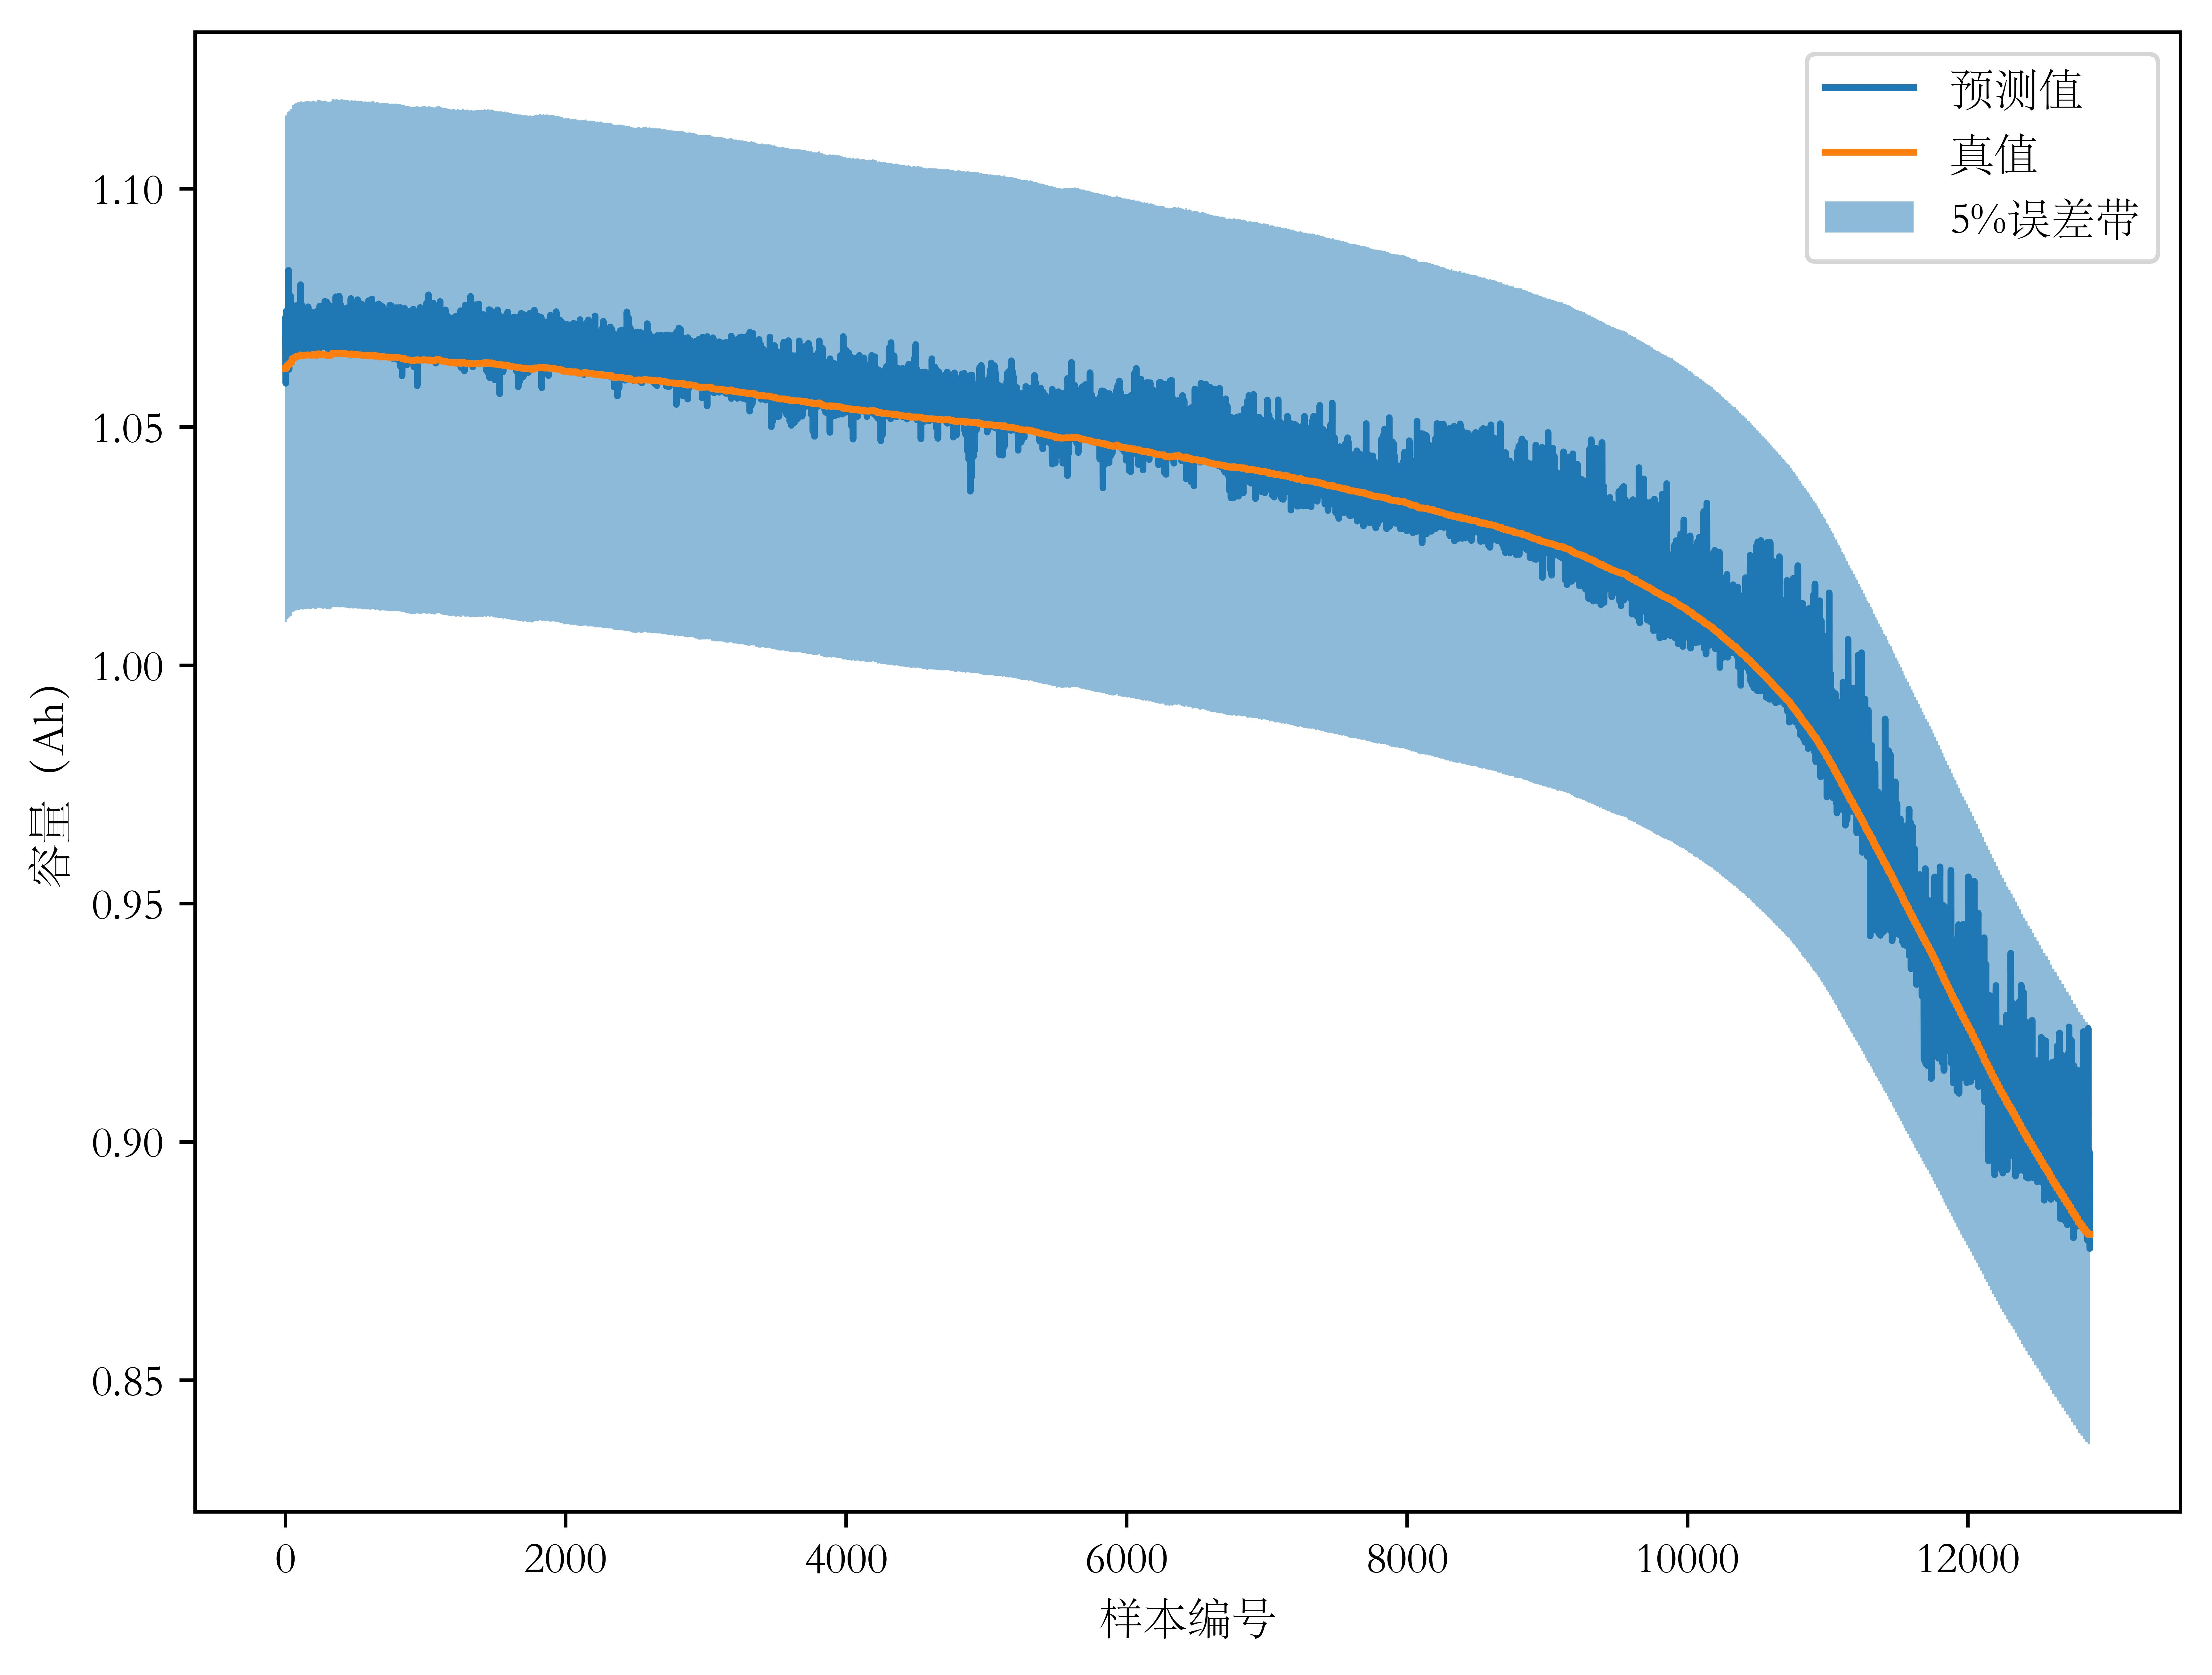
\includegraphics[width=0.25\textwidth]{figures/soh_vitq/tri_group1_cell4_cnn_viq_trans.jpg}}
		\captionsetup{font=tiny}
		\caption{CNN模型在四种不同训练配置下SOH估计结果示意图}
	\end{figure}
	\begin{itemize}
		\item 在TRI数据集(包含16块电池的循环数据,均分为四组)上进行实验,对电池分组采用留一法划分数据集
		\item 受篇幅限制,展示其中编号为b3c0的电池在四种不同实验配置下的测试结果
	\end{itemize}
	\pdfnote{本课题的第二部分是基于充放电过程中直接测量量的电池SOH估计,使用部分充电段数据作为输入,克服了直接使用放电容量的方法的难以在线应用的问题。}
\end{frame}

\begin{frame}
	\begin{table}[]
		\centering
		\resizebox{\columnwidth}{!}{%
			\begin{tabular}{ccccc}
				\toprule
				评价指标   & VIT输入,无变换 & VIT输入,有变换 & VIq输入,无变换 & VIq输入,有变换 \\
				\midrule
				平均MaxE & 0.110514  & 0.131351  & 0.08509   & 0.068284  \\
				平均MAE  & 0.011018  & 0.015671  & 0.006605  & 0.006807  \\
				平均RMSE & 0.016167  & 0.021842  & 0.010835  & 0.009845  \\
				模型参数量  & 60421     & 12693     & 60421     & 12693     \\
				\bottomrule
			\end{tabular}%
		}
		\captionsetup{font=tiny}
		\caption{四组实验CNN模型SOH估计性能评估结果}
	\end{table}
	\begin{itemize}
		\item 对比使用V、I、T为输入的情形,使用V、I、q为输入时模型预测性能有显著提升
		\item 使用时间序列-图像变换能在保持预测精度的前提下显著降低模型参数量
	\end{itemize}
	\pdfnote{这一页展示了CNN模型在四种不同输入配置下的预测性能。\\由此,对比使用V、I、T为输入的情形,使用V、I、q为输入时模型预测性能有显著提升;使用时间序列-图像变换能在保持预测精度的前提下显著降低模型参数量。}
\end{frame}

\subsection{电池RUL预测}

\begin{frame}
	\begin{figure}[htbp]
		\centering
		\subfloat[电池044的RUL预测结果]
		{\label{fig:subfig1}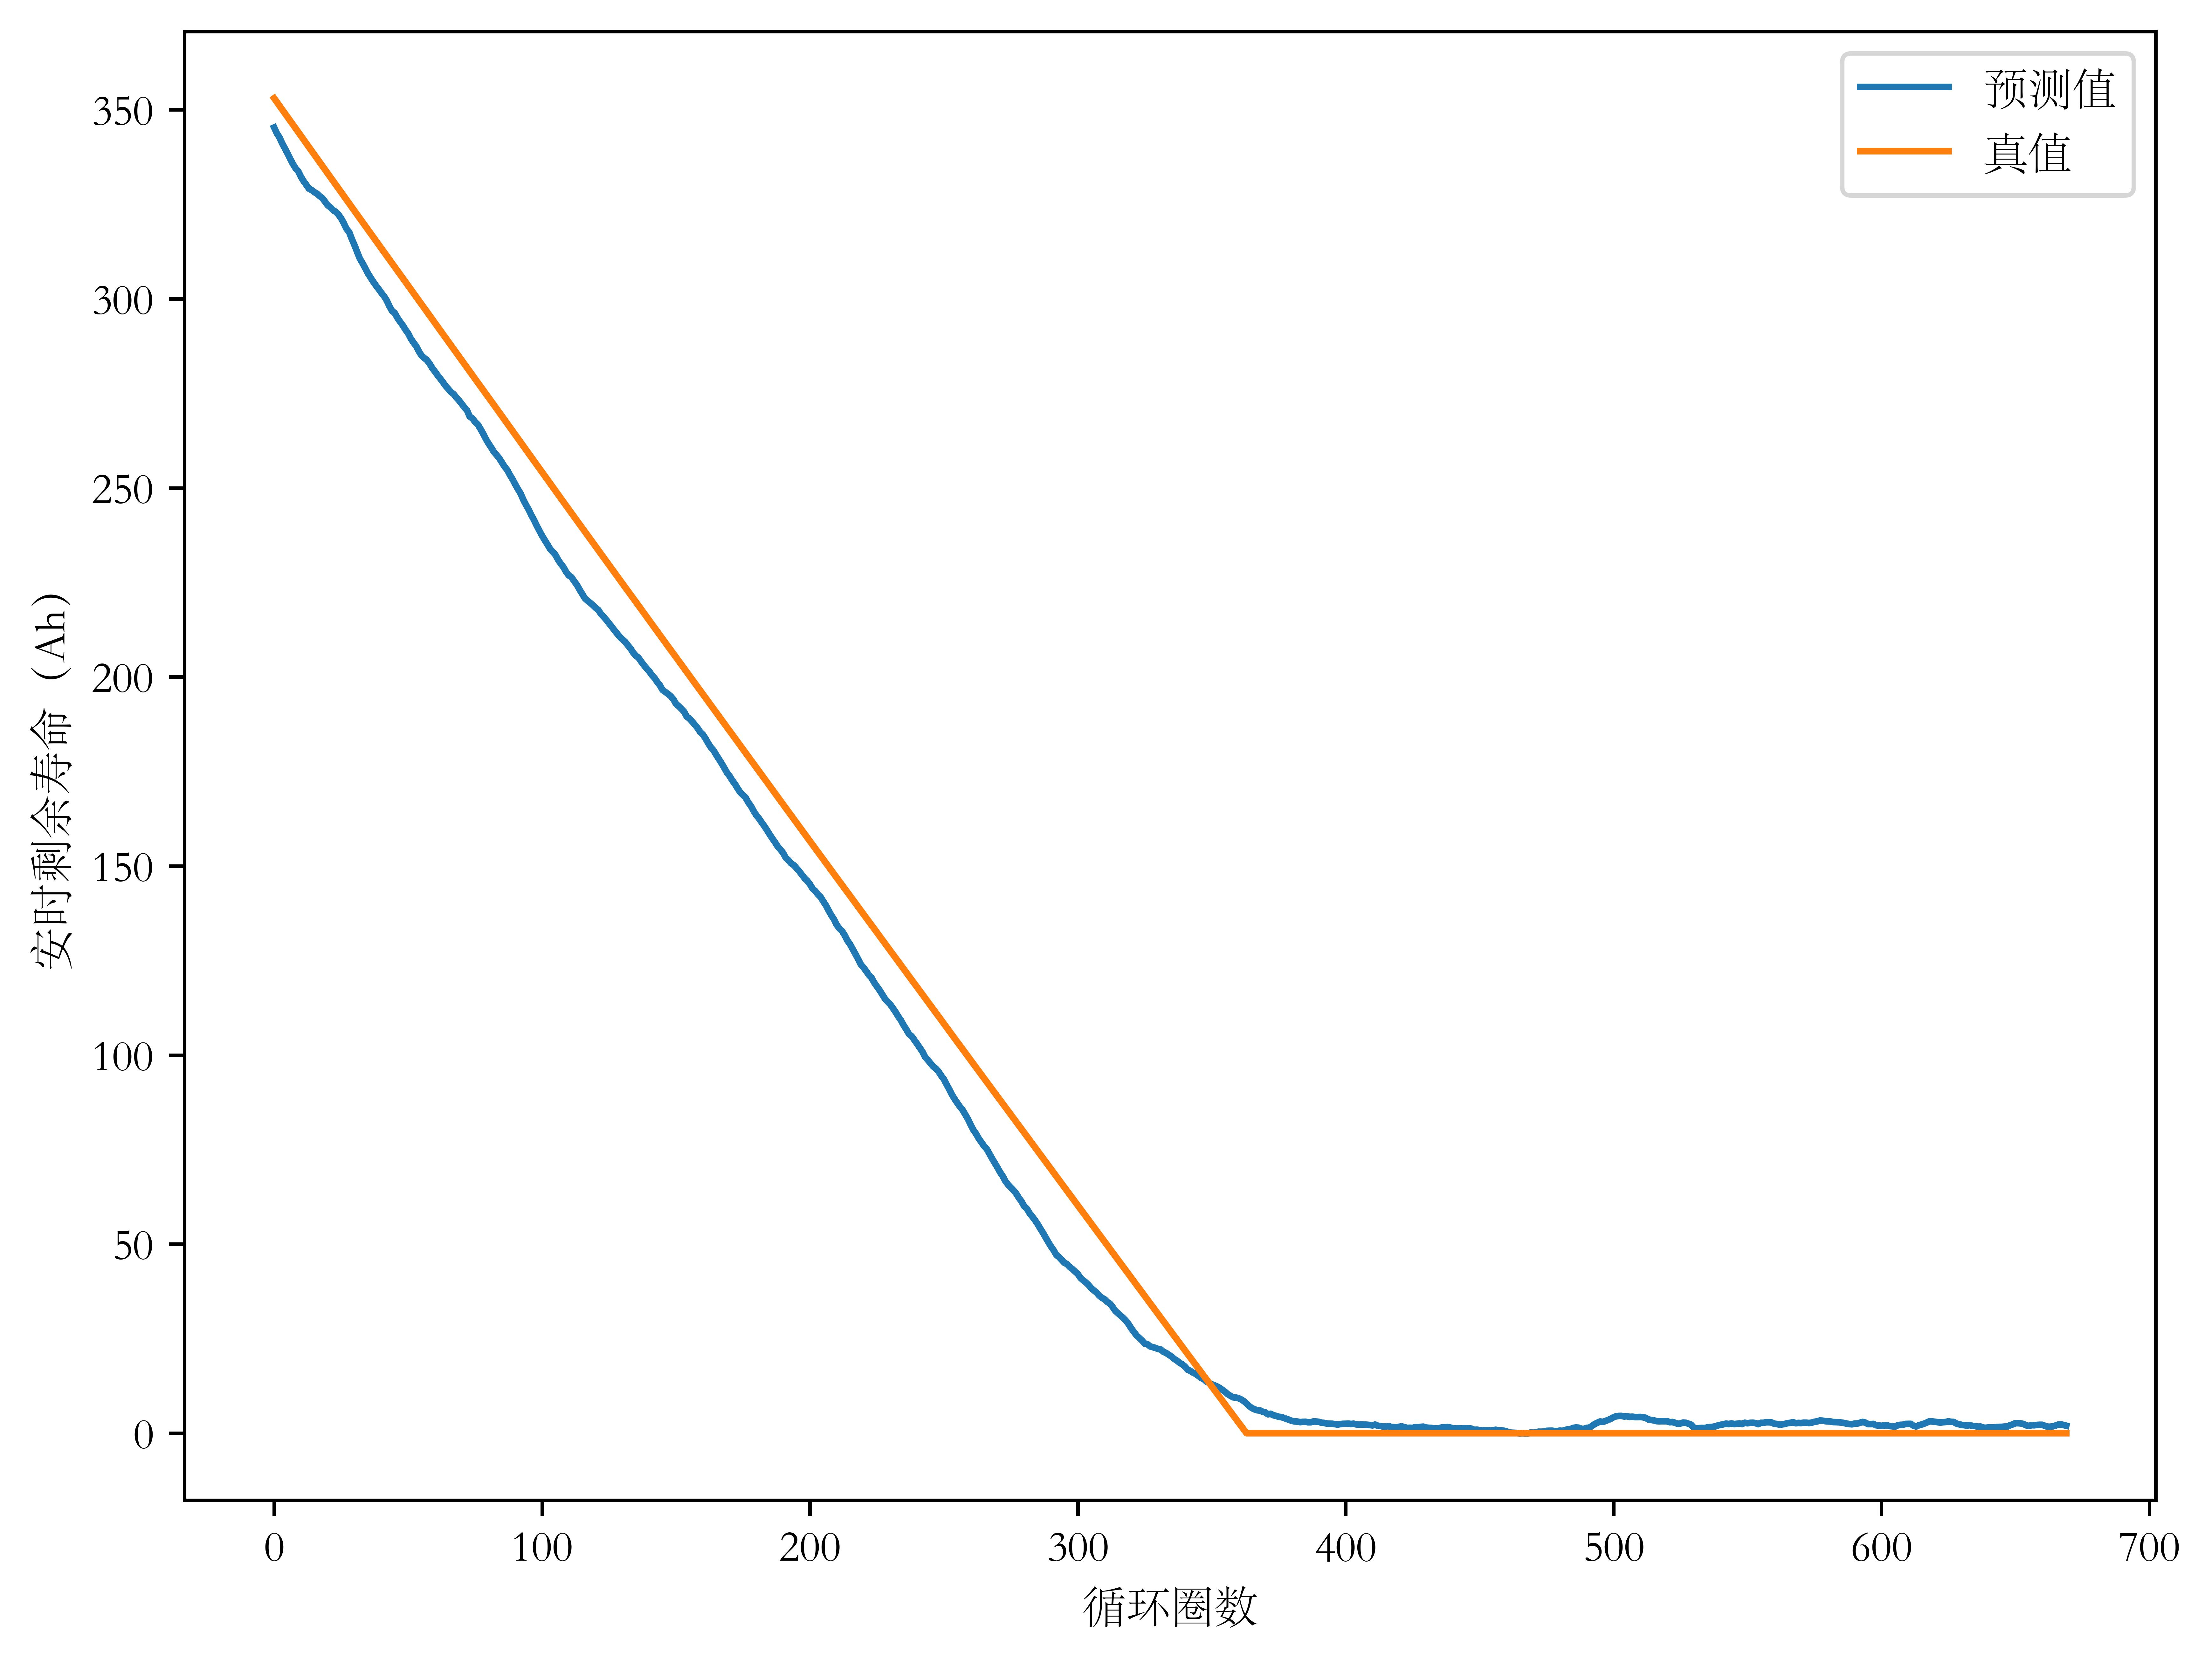
\includegraphics[width=0.3\textwidth]{figures/rul/unibo_lstm_rul_cycle_4.jpg}}
		\subfloat[电池039的RUL预测结果]
		{\label{fig:subfig2}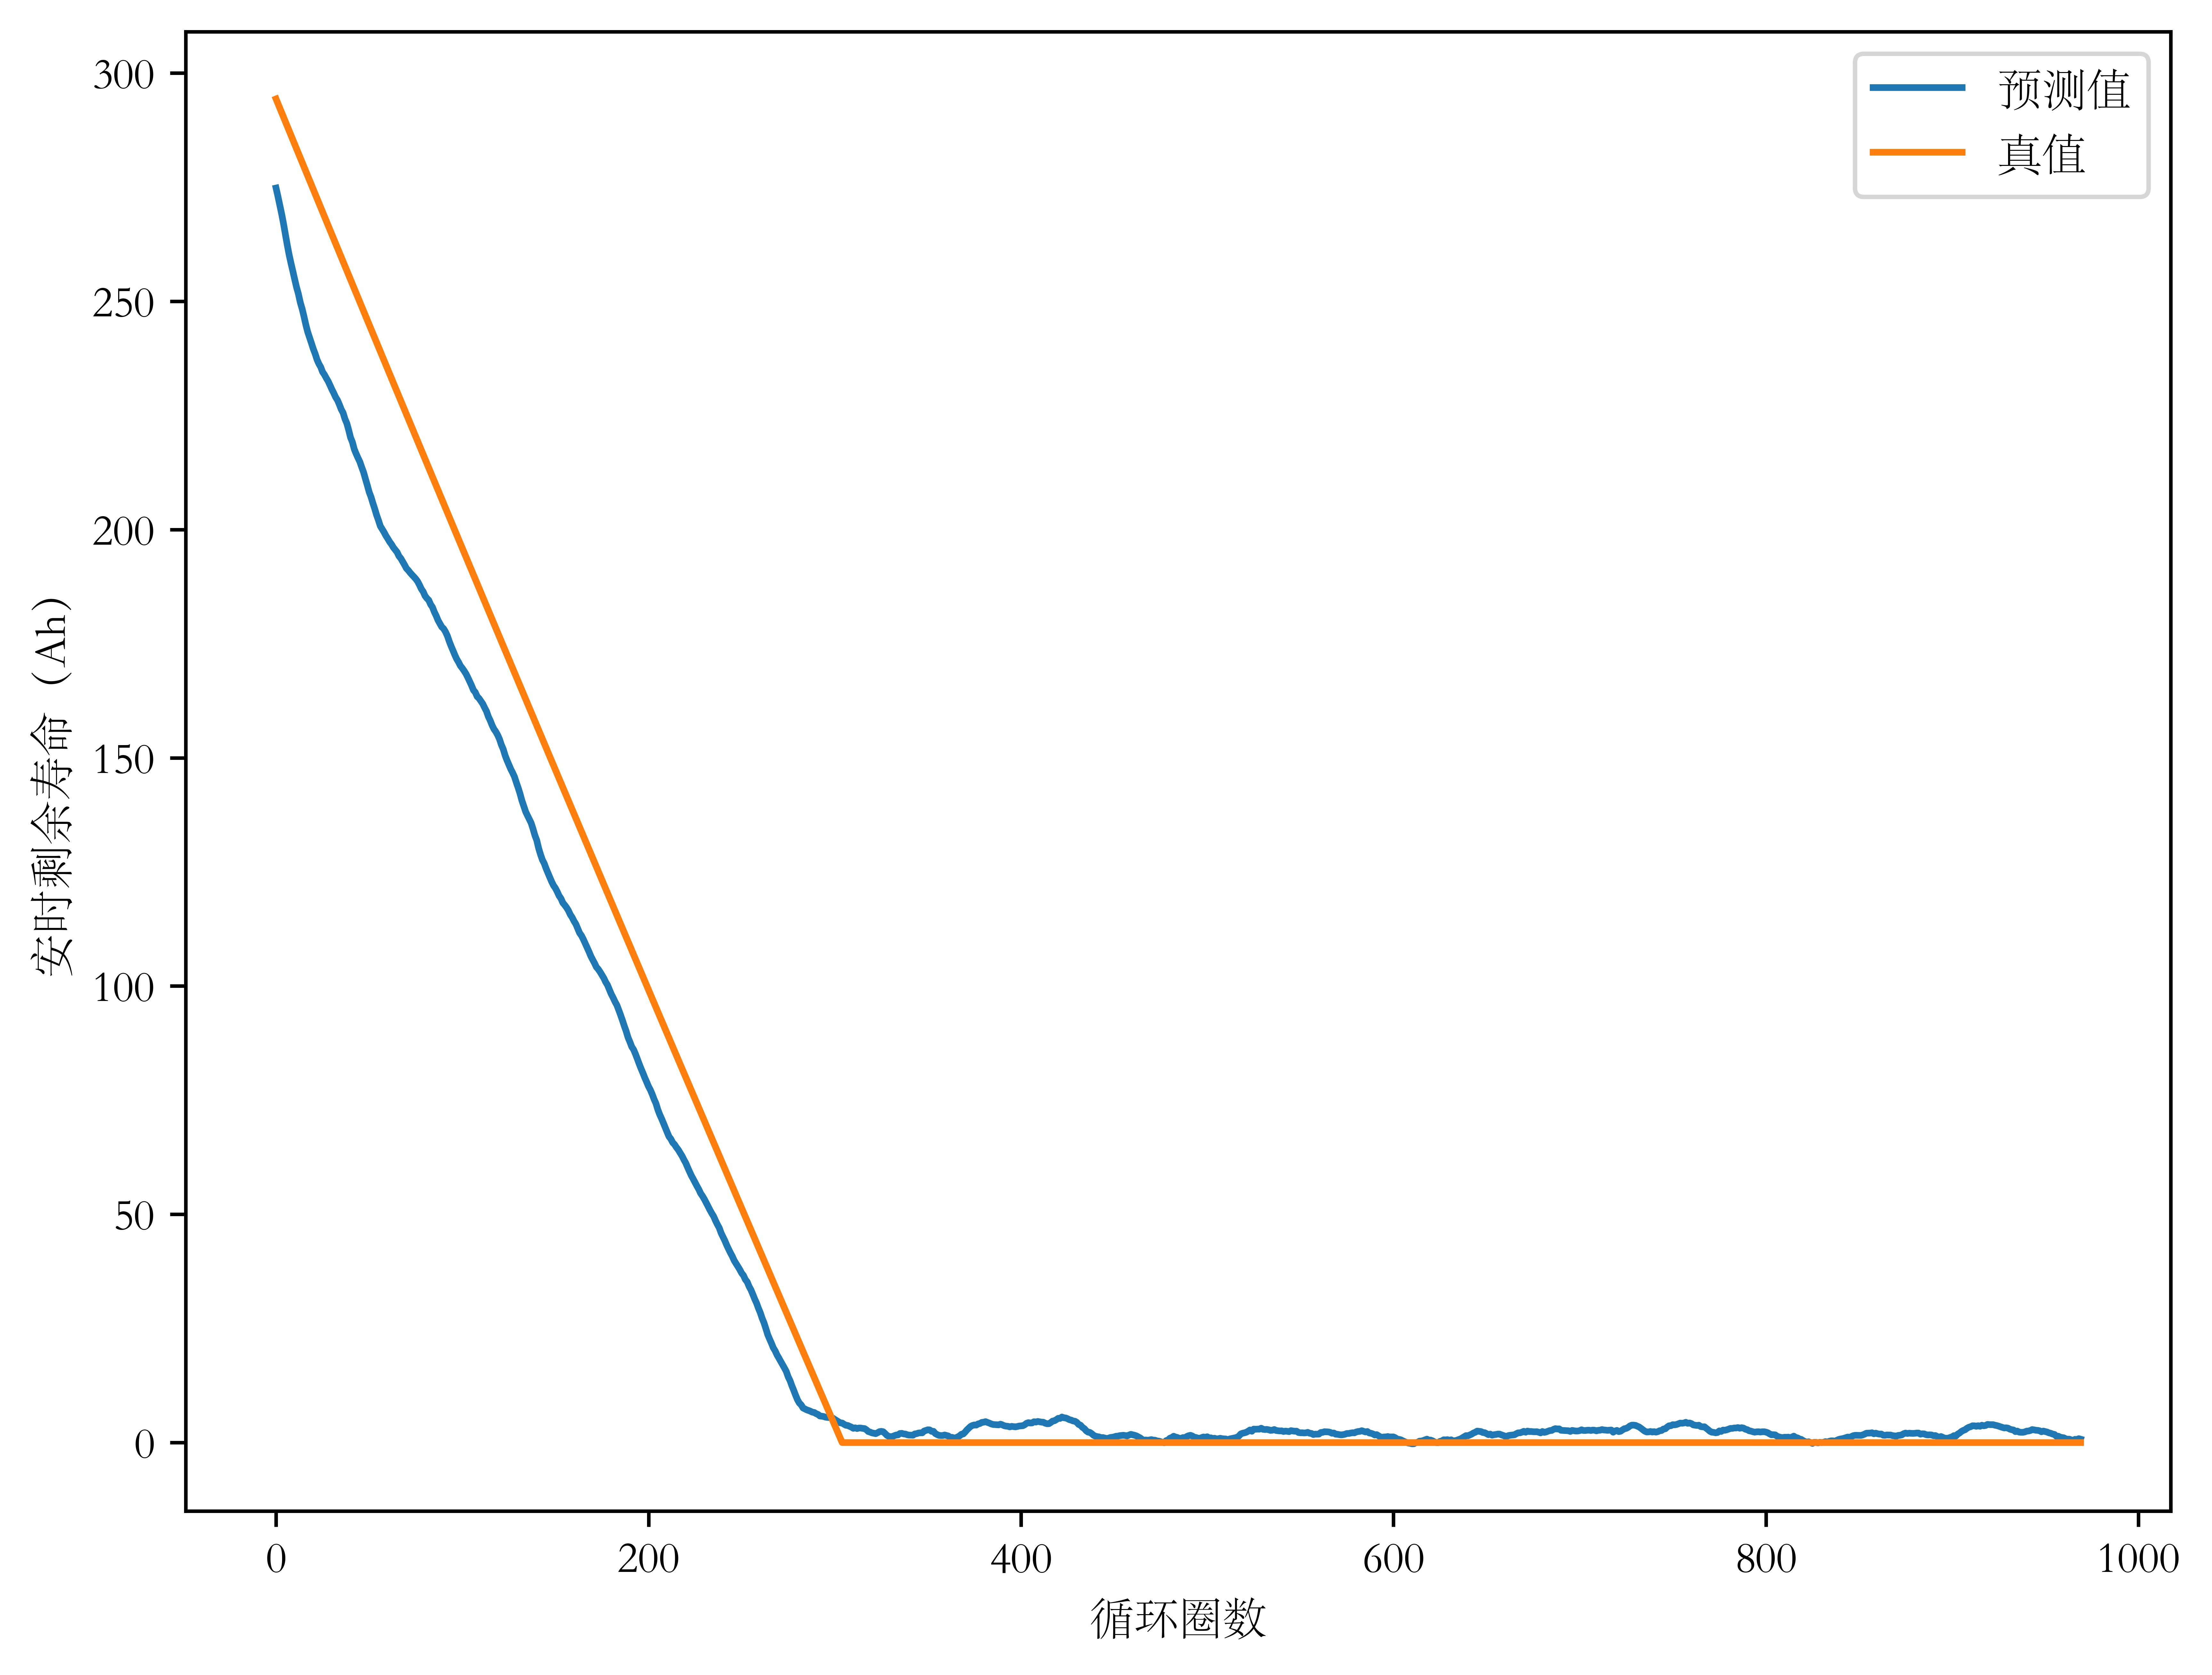
\includegraphics[width=0.3\textwidth]{figures/rul/unibo_lstm_rul_cycle_5.jpg}}
		\subfloat[电池041的RUL预测结果]
		{\label{fig:subfig3}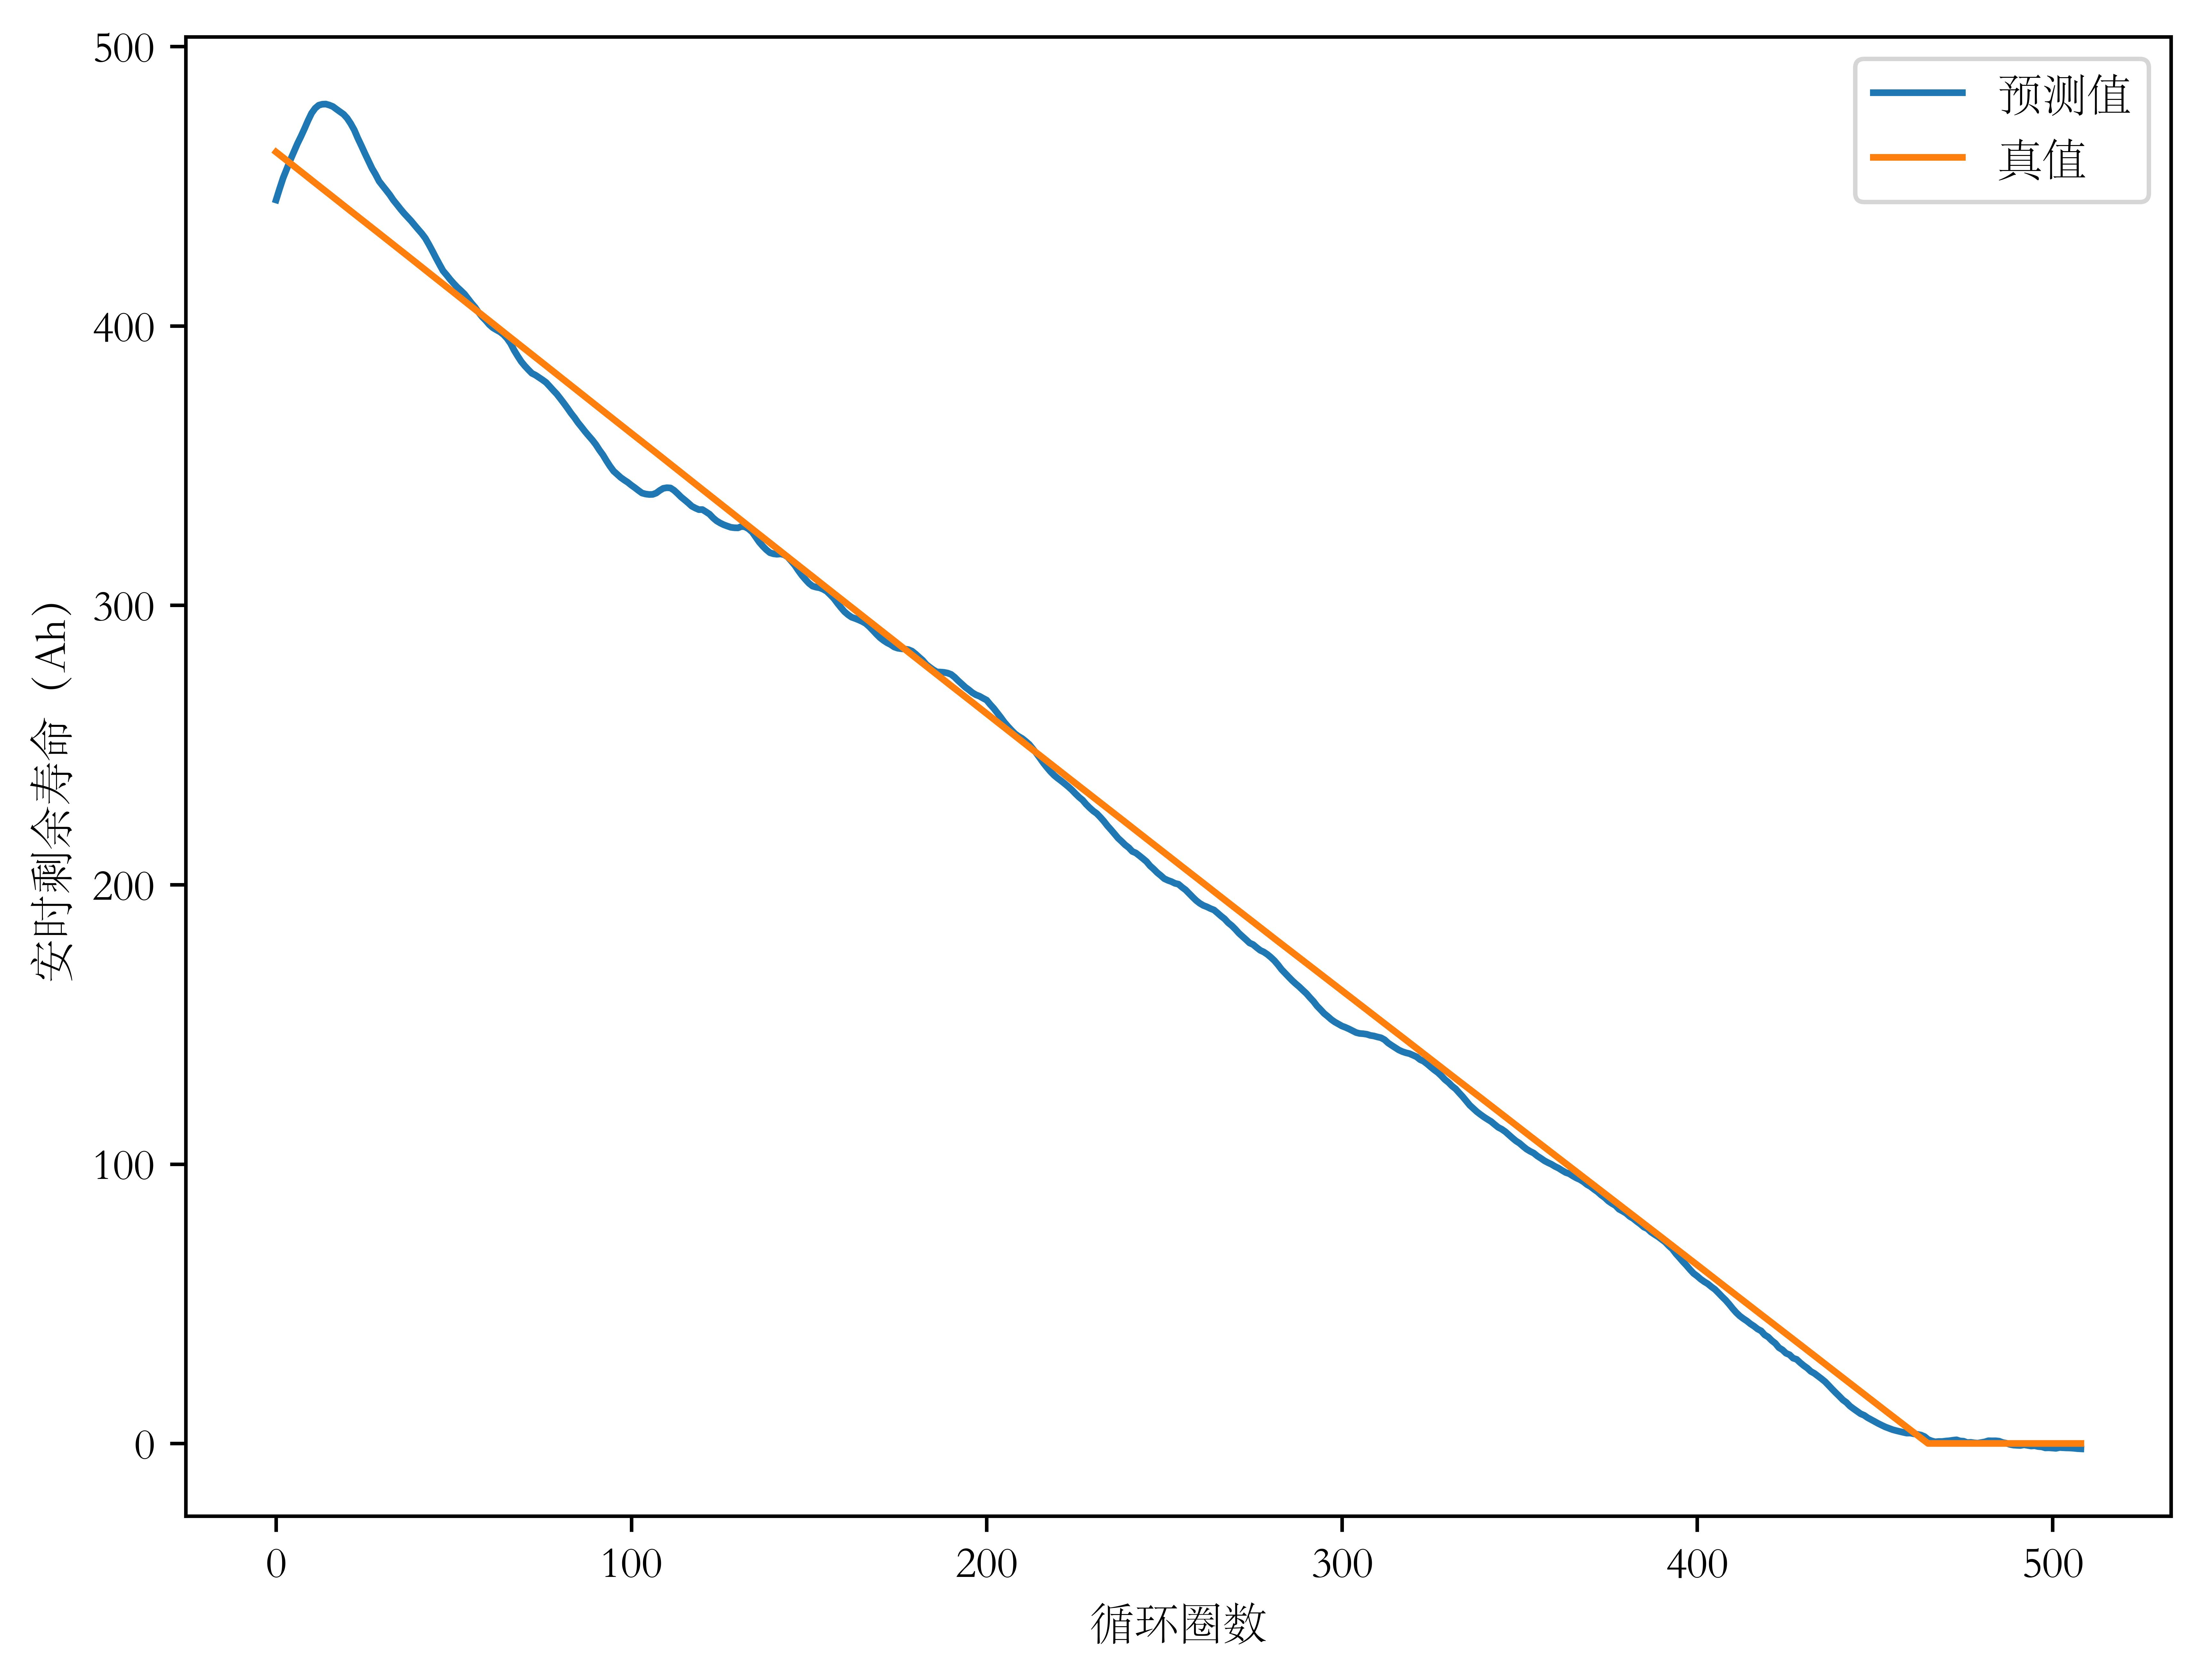
\includegraphics[width=0.3\textwidth]{figures/rul/unibo_lstm_rul_cycle_6.jpg}}
		\captionsetup{font=tiny}
		\caption{DeepLSTM模型的RUL预测结果示意图}
	\end{figure}
	\begin{itemize}
		\item 在Unibo Powertools数据集(包含27块电池的循环数据)上进行实验,其中20块电池数据用作训练集、7块电池数据被用作测试集
		\item 受篇幅限制,展示在编号为044、039和041的电池上的测试结果
	\end{itemize}
	\pdfnote{以上述两个部分对电池SOH的研究为基础,本课题第三部分研究电池RUL预测问题。}
\end{frame}

\begin{frame}
	\begin{table}[]
		\centering
		\resizebox{\columnwidth}{!}{%
			\begin{tabular}{ccccccccc}
				\toprule
				评价指标  & 电池003    & 电池011    & 电池013    & 电池006    & 电池044    & 电池039    & 电池041    & 均值       \\
				\midrule
				RMSE  & 3.855191 & 3.102227 & 10.77393 & 10.12258 & 13.87137 & 8.883196 & 4.498271 & 7.872395 \\
				NRMSE & 0.035861 & 0.02924  & 0.181346 & 0.028673 & 0.047128 & 0.019219 & 0.051681 & 0.056164 \\
				\bottomrule
			\end{tabular}%
		}
		\captionsetup{font=tiny}
		\caption{DeepLSTM模型电池Ah-RUL预测性能}
	\end{table}
	\begin{itemize}
		\item 实验结果表明使用数据驱动方法实现锂离子电池RUL预测具有可行性
	\end{itemize}
	\pdfnote{这一页展示了深度LSTM模型在测试集的7块电池上的预测性能。\\实验结果证明了使用数据驱动方法实现电池RUL预测的可行性。}
\end{frame}

\section{总结与展望}

\begin{frame}
	\begin{itemize}
		\item 总结
		      \begin{itemize}
			      \item 基于电池容量历史退化数据实现SOH估计,比较五种模型的预测性能
			      \item 基于电池充放电直接测量量实现SOH估计,使用电荷量取代电池表面温度作为模型输入提高预测性能,使用时间序列-图像变换减少模型参数量
			      \item 基于电池充放电直接测量量实现RUL预测,提出依据容量定义的Ah-RUL取代依据循环圈数定义的cycle-RUL
		      \end{itemize}
		\item 展望
		      \begin{itemize}
			      \item 估计/预测模型改进
			            \begin{itemize}
				            \item 研究融合模型,提高预测性能
				            \item 引入贝叶斯方法,实现对预测结果的不确定性度量以更好支持工业决策
				            \item 引入迁移学习策略,提高模型泛化能力
			            \end{itemize}
			      \item 模型在嵌入式平台的部署:模型量化和模型转换
		      \end{itemize}
	\end{itemize}
	\pdfnote{以上是本课题的主要研究内容,第一、二部分研究电池SOH估计问题,第三部分研究电池RUL预测问题。\\以下两方面工作是我未来的研究方向,其一,针对估计/预测模型,可以通过模型融合提高预测性能,可以引入贝叶斯方法对回归结果进行不确定性度量,可以通过引入迁移学习策略提高模型的泛化能力;其二,针对模型在实际车机系统上的部署,需要解决模型量化和模型转换的问题。}
\end{frame}

\section{写在最后}

\subsection{代码可用性}

\begin{frame}
	\centering
	本课题相关代码已在github上开源,请见:

	\centering
	\url {https://github.com/hilinxinhui/battery_phm.git}

	\begin{figure}[htbp]
		\centering
		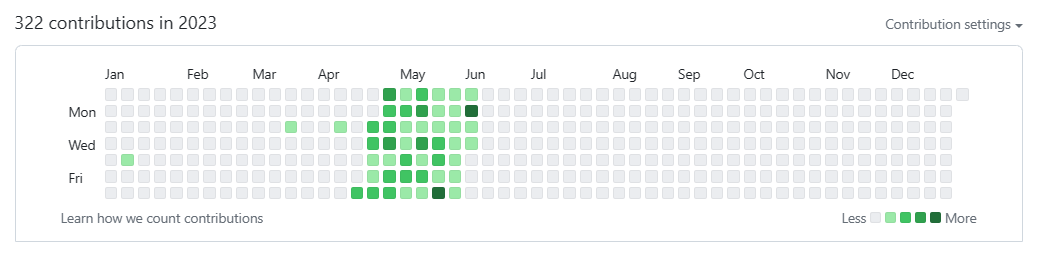
\includegraphics[scale=0.35]{figures/github_contribution_log.png}
	\end{figure}

	\begin{figure}[htbp]
		\centering
		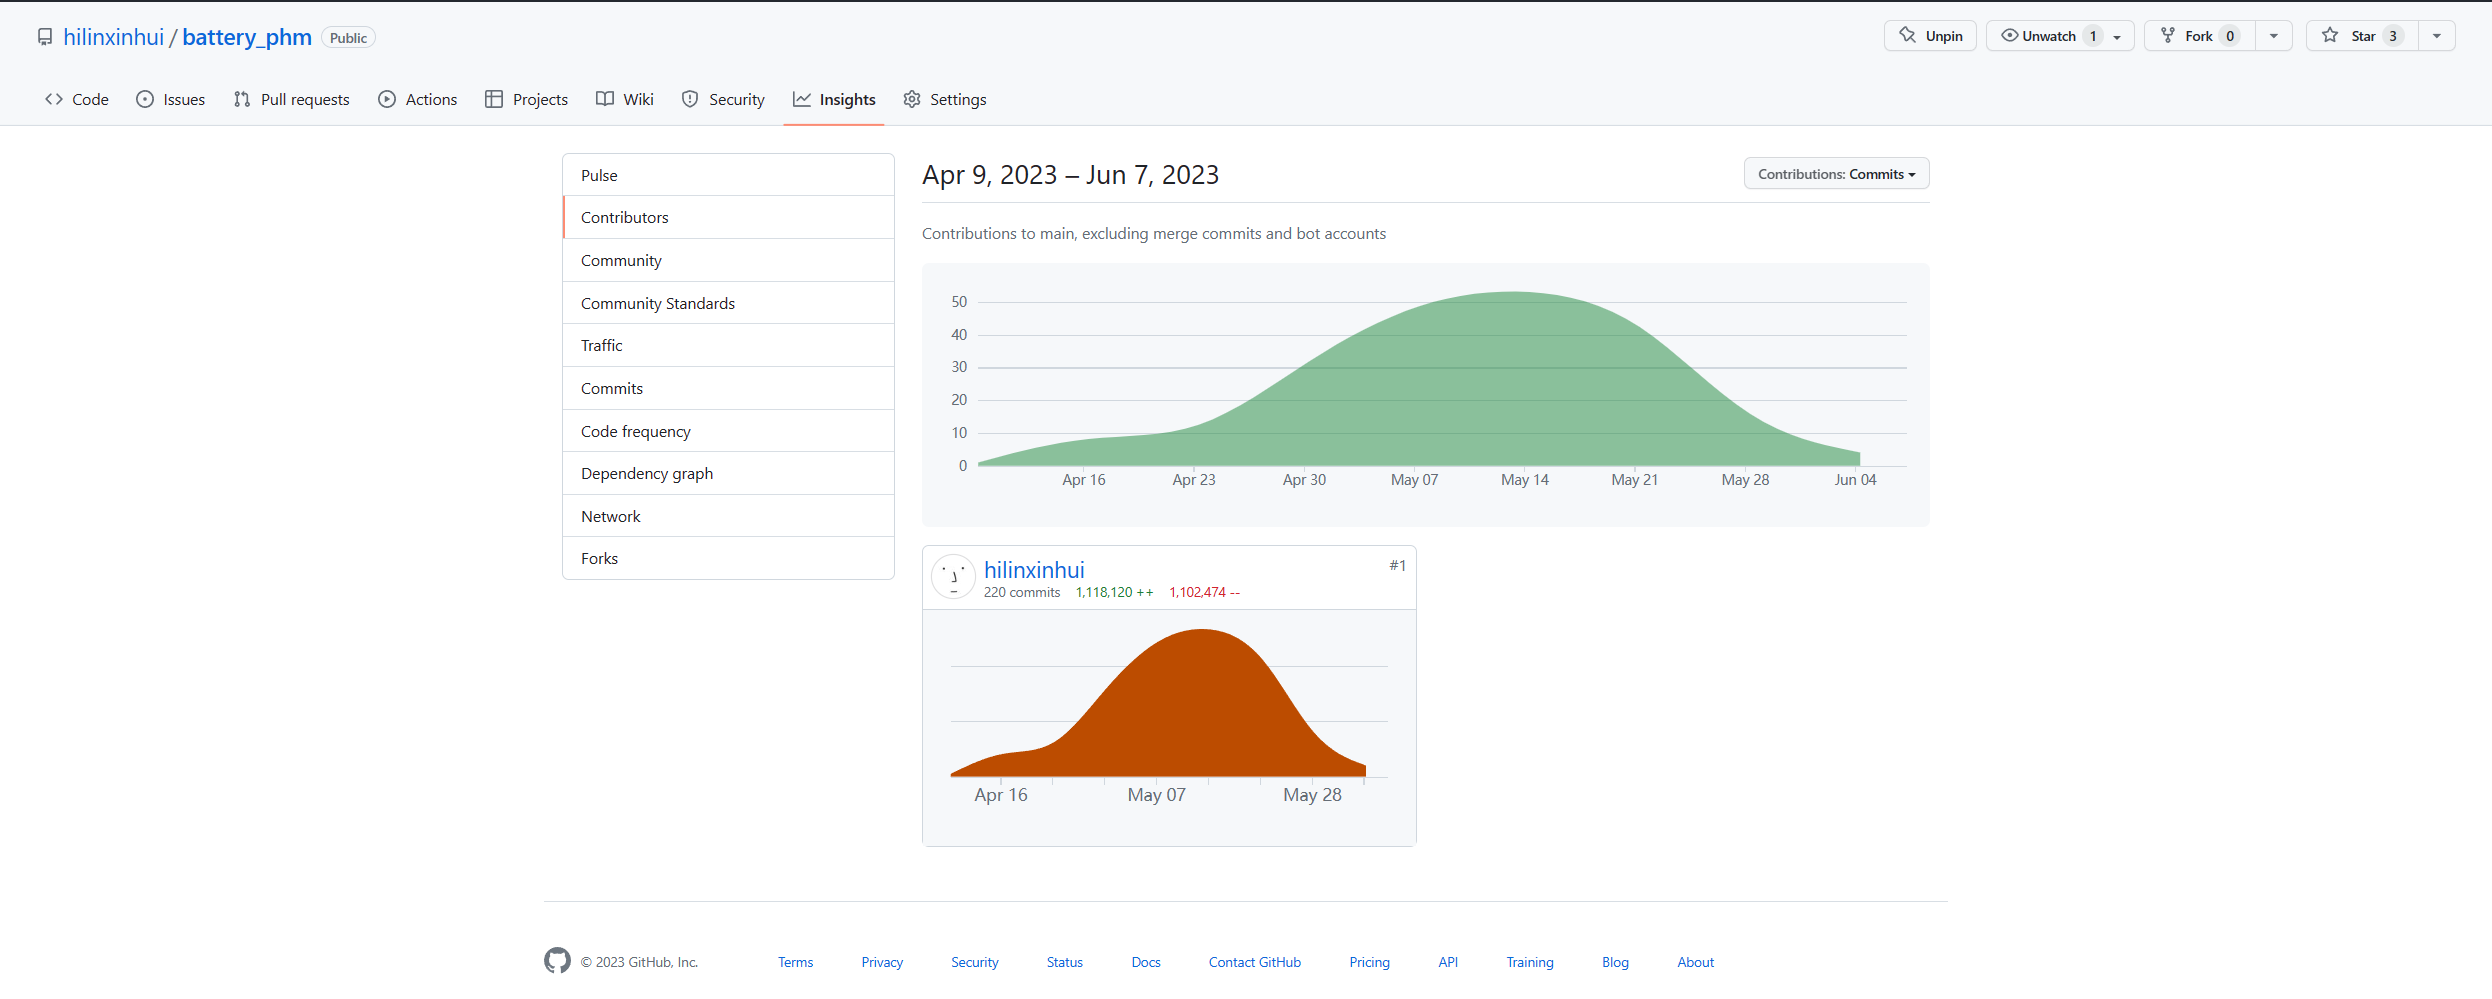
\includegraphics[scale=0.15]{figures/github_contribution_log_2.png}
	\end{figure}

\end{frame}

\subsection{感谢各位老师}

\begin{frame}
	\LARGE \centering 汇报完毕,请各位老师批评指正!
    \note{我的汇报到此结束,感谢各位老师的耐心倾听,请老师批评指正。}
\end{frame}

\end{document}
